%!TEX root = ../thesis.tex
%*******************************************************************************
%******************************* Introduction **********************************
%*******************************************************************************

% To use nomenclature, see README.md: run Tools > User > makenomenclature
\nomenclature[i-ERC]{ERC}{European Research Council}
\nomenclature[i-MERAC]{MERAC}{Mobilising European Research in Astrophysics and Cosmology}
\nomenclature[i-NWO]{NWO}{Nederlandse Organisatie voor Wetenschappelijk Onderzoek (Dutch Research Council)}
\nomenclature[i-STFC]{STFC}{Science and Technology Facilities Council}
\nomenclature[i-ESO]{ESO}{European Southern Observatory}
\nomenclature[i-NRAO]{NRAO}{National Radio Astronomy Observatory}
\nomenclature[i-NAOJ]{NAOJ}{National Astronomical Observatory of Japan}
\nomenclature[i-STScI]{STScI}{Space Telescope Science Institute}
\nomenclature[i-ESA]{ESA}{European Space Agency}
\nomenclature[i-NASA]{NASA}{National Aeronautics and Space Administration}
\nomenclature[i-MAST]{MAST}{Barbara A. Mikulski Archive for Space Telescopes}

\nomenclature[j-AandA]{A\&A(Rv)}{Astronomy and Astrophysics (Review)}
\nomenclature[j-AJ]{AJ}{Astronomical Journal}
\nomenclature[j-ApJ]{ApJ(S)}{Astrophysical Journal (Supplement)}
\nomenclature[j-ARAandA]{ARA\&A}{Annual Review of Astronomy and Astrophysics}
\nomenclature[j-MNRAS]{MNRAS}{Monthly Notices of the Royal Astronomical Society}
\nomenclature[j-NA]{New~Astron.}{New Astronomy}
\nomenclature[j-PASA]{Publ. Astron. Soc. Australia}{Publications of the Astronomical Society of Australia}
\nomenclature[j-PASP]{PASP}{Publications of the Astronomical Society of the Pacific}
\nomenclature[j-PASJ]{PASJ}{Publications of the Astronomical Society of Japan}
\nomenclature[j-RMxAA]{Phys. Rev.~(A-E/Lett.)}{Physical Review (A-E/Letters)}
\nomenclature[j-PR]{Phys.~Rep.}{Physics Reports}
\nomenclature[j-RMxAA]{Rev. Mex. Astron. Astrofis.}{Revista Mexicana de Astronomia y Astrofisica}
\nomenclature[j-ZAP]{Z.~Astrophys.}{Zeitschrift f{\"u}r Astrophysik}

\nomenclature[a-a]{$a$}{scale factor}
\nomenclature[a-A]{$A$}{area (or spontaneous emission coefficient, e.g. $A_{21}$, or extinction, e.g. $A_V$)}
\nomenclature[a-Bnu]{$B_\nu$}{\citeauthor{1901AnP...309..553P} function, described by \cref{chIeq:Planck_function}}
\nomenclature[a-C]{$C$}{clumping factor (or collisional transition coefficients, e.g. $C_{12}$)}
\nomenclature[a-d]{$d$}{distance (e.g. $d_L$ the luminosity distance, $d_A$ the angular-diameter distance)}
\nomenclature[a-E]{$E$}{energy}
\nomenclature[a-f]{$f$}{fraction: $f_\text{esc}$ the escape fraction or $f_\text{rec, A/B}$ the (case-A/B) recombination fraction (\cref{appPsec:Model parameters})}
\nomenclature[a-F]{$F$}{flux ($F_\nu$ or $F_\lambda$ the flux density)}
\nomenclature[a-g]{$g$}{degeneracy factor (or $g_{\mu \nu}$ the metric)}
\nomenclature[a-H]{$H$}{Hubble parameter ($H_0$ the Hubble constant)}
\nomenclature[a-Inu]{$I_\nu$}{specific intensity}
\nomenclature[a-J]{$J_\nu$}{specific intensity (of an isotropic radiation field)}
\nomenclature[a-K]{$K$}{curvature parameter ($K \in \{ -1, 0, 1 \}$)}
\nomenclature[a-l]{$l$}{length}
\nomenclature[a-L]{$L$}{luminosity}
\nomenclature[a-m]{$m$}{particle mass}
\nomenclature[a-M]{$M$}{object mass (e.g. $M_\text{J}$ the \citeauthor{1902RSPTA.199....1J} mass)}
\nomenclature[a-n]{$n$}{number density (e.g. $n_\text{H}$ the hydrogen number density)}
\nomenclature[a-N]{$N$}{column density or number (e.g. $\dot{N}_\text{ion}$ the number of ionising photons per unit time)}
\nomenclature[a-p]{$P$}{pressure}
\nomenclature[a-qion]{$q_\text{ion}$}{ionisation parameter, defined in \cref{chIeq:Ionisation_parameter}}
\nomenclature[a-r]{$r$}{radial coordinate or radius}
\nomenclature[a-R]{$R$}{specific radius (e.g. $R_\text{vir}$ the virial radius), $R_{\mu \nu}$ the Ricci tensor, $R_V$ the extinction slope, or $R \equiv \lambda/\Delta \lambda$ the spectral resolution}
\nomenclature[a-Snu]{$S_\nu$}{flux density (see $F_\nu$)}
\nomenclature[a-t]{$t$}{time (or timescale, e.g. $t_\text{cool}$)}
\nomenclature[a-T]{$T$}{temperature or atmospheric transmission (or $T^{\mu \nu}$ the energy-momentum tensor)}
\nomenclature[a-U]{$U$}{normalised ionisation parameter, $U = q_\text{ion} / c$}
\nomenclature[a-v]{$v$}{velocity}
\nomenclature[a-V]{$V$}{volume}
\nomenclature[a-w]{$w$}{equation of state, $w \equiv P/\rho c^2$}
\nomenclature[a-x]{$x$}{coordinate along $x$-axis ($\vec{x}$ physical coordinates)}
\nomenclature[a-X]{$X$}{fraction (e.g. $X_\text{\ion{H}{I}}$ the neutral hydrogen fraction) or factor (e.g. $X_\mathrm{\upalpha/Fe, \, neb}$ the $\mathrm{\upalpha/Fe}$ enhancement factor)}
\nomenclature[a-y]{$y$}{coordinate along $y$-axis (or yield, e.g. $y_\text{dust, SN}$)}
\nomenclature[a-z]{$z$}{redshift, defined in \cref{chIeq:Redshift}}
\nomenclature[a-Z]{$Z$}{metallicity, defined in \cref{chIeq:Metallicity}}

\nomenclature[a-alpha]{$\alpha$}{right ascension, power-law exponent, or $\alpha_\text{A/B}$ the (case-A/B) recombination coefficient (\cref{appPsec:Model parameters})}
\nomenclature[a-beta]{$\beta$}{$\beta_\text{UV}$ the UV slope, $\beta_\text{IR}$ the dust emissivity}
\nomenclature[a-gamma]{$\gamma$}{$\gamma_\text{1s2p}$ the specific collisional excitation coefficient for collisional excitation of \lya\ (\cref{appPsec:Model parameters})}
\nomenclature[a-delta]{$\delta$}{declination or overdensity}
\nomenclature[a-Delta]{$\Delta$}{overdensity (or difference, e.g. $\Delta_\text{FMR} ( 12 + \log ( \text{O/H} ))$)}
\nomenclature[a-eps]{$\epsilon$}{emissivity ($\epsilon_\nu$ the specific emissivity)}
\nomenclature[a-eta]{$\eta$}{efficiency factor}
\nomenclature[a-theta]{$\theta$}{polar angle coordinate (or IMF power-law exponent)}
\nomenclature[a-kappa]{$\kappa$}{$\kappa_\nu$ the dust absorption cross section (per unit mass)}
\nomenclature[a-lambda]{$\lambda$}{wavelength (e.g. $\lambda_\text{emit}$ the rest-frame wavelength, $\lambda_\text{obs}$ the observed wavelength)}
\nomenclature[a-Lambda]{$\Lambda$}{cosmological constant or $\Lambda (T)$ the cooling function}
\nomenclature[a-mu]{$\mu$}{mean molecular weight, $\mu = m / m_\text{p}$, or magnification factor}
\nomenclature[a-nu]{$\nu$}{frequency (e.g. $\nu_\text{emit}$ the rest-frame frequency, $\nu_\text{obs}$ the observed frequency)}
\nomenclature[a-xi]{$\xi$}{$\xi (M)$ the IMF or $\xi_\text{ion}$ the LyC photon production efficiency}
\nomenclature[a-rho]{$\rho$}{density ($\rho_\text{UV}$ the UV luminosity density, $\rho_\text{SFR}$ the SFR density)}
\nomenclature[a-sigma]{$\sigma$}{velocity dispersion or standard deviation}
\nomenclature[a-Sigma]{$\Sigma$}{surface density ($\Sigma_\text{dust}$ dust surface mass density)}
\nomenclature[a-tau]{$\tau$}{timescale or $\tau (\nu)$ the optical depth}
\nomenclature[a-phi]{$\phi$}{azimuthal angle coordinate}
\nomenclature[a-chi]{$\chi$}{comoving radial geodesic distance ($\vec{\chi}$ comoving coordinates)}
\nomenclature[a-omega]{$\omega$}{angular frequency or $\dif \omega$ the solid angle element}
\nomenclature[a-Omega]{$\Omega$}{density parameter, $\Omega = \rho / \rho_\text{crit}$, or solid angle}

\nomenclature[c-pi]{$\pi = \num{3.14159}\dots$}{mathematical constant}
\nomenclature[c-G]{$G \simeq 6.674 \cdot 10^{-11} \, \mathrm{m^3 \, kg^{-1} \, s^{-2}}$}{gravitational constant}
\nomenclature[c-c]{$c = \num{299792458} \, \mathrm{m \, s^{-1}}$}{speed of light}
\nomenclature[c-kb]{$k_\text{B} = \num{1.380649} \cdot 10^{-23} \, \mathrm{J \, K^{-1}}$}{Boltzmann constant}
\nomenclature[c-mp]{$m_\text{p} \simeq 1.673 \cdot 10^{-27} \, \mathrm{kg}$}{proton mass}
\nomenclature[c-h]{$h = \num{6.62607015} \cdot 10^{-34} \, \mathrm{J \, Hz^{-1}}$}{Planck constant}

\nomenclature[d-LyC]{LyC}{Lyman continuum}
\nomenclature[d-UV]{UV}{ultraviolet}
\nomenclature[d-IRX]{IR(X)}{infrared (excess)}
\nomenclature[d-NIR]{NIR}{near infrared}
\nomenclature[d-MIR]{MIR}{mid infrared}
\nomenclature[d-FIR]{FIR}{far infrared}
\nomenclature[d-Lya]{\lya}{\lymana}

\nomenclature[d-GR]{GR}{General Relativity}
\nomenclature[d-CDM]{CDM}{cold dark matter (see also \LCDM)}
\nomenclature[d-LCDM]{\LCDM}{$\Lambda$ cold dark matter (see also CDM)}
\nomenclature[d-CMB]{CMB}{cosmic microwave background}
\nomenclature[d-SN]{SN}{supernova}
\nomenclature[d-BBN]{BBN}{Big Bang Nucleosynthesis}
\nomenclature[d-BAO]{BAO}{baryon acoustic oscillations}
\nomenclature[d-UVB]{UVB}{ultraviolet background}
\nomenclature[d-GMC]{GMC}{giant molecular cloud}
\nomenclature[d-sSFR]{(s)SFR}{(specific) star formation rate}
\nomenclature[d-IMF]{IMF}{initial mass function}
\nomenclature[d-AGB]{AGB}{asymptotic giant branch}
\nomenclature[d-MZR]{MZR}{mass-metallicity relation}
\nomenclature[d-FMR]{FMR}{Fundamental Metallicity Relation}
\nomenclature[d-ISM]{ISM}{interstellar medium}
\nomenclature[d-IGM]{IGM}{intergalactic medium}
\nomenclature[d-CGM]{CGM}{circumgalactic medium}
\nomenclature[d-EoR]{EoR}{Epoch of Reionisation}
\nomenclature[d-PDR]{PDR}{photodissociation region}
\nomenclature[d-LBG]{LBG}{Lyman-break galaxy}
\nomenclature[d-SED]{SED}{spectral energy distribution}
\nomenclature[d-EW]{EW}{equivalent width}
\nomenclature[d-RA]{RA}{right ascension}
\nomenclature[d-Dec]{Dec}{declination}
\nomenclature[d-SB]{SB}{surface brightness}
\nomenclature[d-PWV]{PWV}{precipitable water vapour}
\nomenclature[d-MFP]{MFP}{mean free path}
\nomenclature[d-IFU]{IFU}{integral field unit}
\nomenclature[d-LAE]{LAE}{\lya\ emitter}
\nomenclature[d-SPH]{SPH}{smoothed particle hydrodynamics}
\nomenclature[d-FoV]{FoV}{field of view}
\nomenclature[d-PSF]{PSF}{point spread function}
\nomenclature[d-FWHM]{FWHM}{full width at half maximum}
\nomenclature[d-VIS]{VIS}{visible}
\nomenclature[d-OB]{OB}{observing block}
\nomenclature[d-SNR]{SNR}{signal-to-noise ratio}
\nomenclature[d-PI]{PI}{principal investigator}
\nomenclature[d-GO]{GO}{general observer}
\nomenclature[d-SF]{SF}{star formation}
\nomenclature[d-SMC]{SMC}{Small Magellanic Cloud}
\nomenclature[d-GP]{GP}{green pea}
\nomenclature[d-ETC]{ETC}{exposure time calculator}
\nomenclature[d-RMS]{RMS}{root mean square}
\nomenclature[d-XDR]{XDR}{X-ray dominated region}
\nomenclature[d-QSO]{QSO}{quasi-stellar object (quasar)}
\nomenclature[d-LIRG]{LIRG}{luminous infrared galaxy (see also ULIRG and HyLIRG)}
\nomenclature[d-ULIRG]{ULIRG}{ultra-luminous infrared galaxy (see also LIRG)}
\nomenclature[d-HyLIRG]{HyLIRG}{hyper-luminous infrared galaxy (see also LIRG)}
\nomenclature[d-SMG]{SMG}{submillimetre galaxy}
\nomenclature[d-LMC]{LMC}{Large Magellanic Cloud}
\nomenclature[d-RJ]{RJ}{Rayleigh-Jeans}
\nomenclature[d-GTO]{GTO}{guaranteed time observations}
\nomenclature[d-BPT]{\citetalias{1981PASP...93....5B}}{\citet*{1981PASP...93....5B}}
\nomenclature[d-HM12]{\citetalias{2019A&ARv..27....3M}}{\citet*{2019A&ARv..27....3M}}
\nomenclature[d-HM12]{\citetalias{2012ApJ...746..125H}}{\citet*{2012ApJ...746..125H}}
\nomenclature[d-P19]{\citetalias{2019MNRAS.485...47P}}{\citet*{2019MNRAS.485...47P}}

\nomenclature[f-JWST]{\textit{JWST}}{\textit{Joris Witstok's favourite Space Telescope}}
\nomenclature[f-HST]{\textit{HST}}{\textit{Hubble Space Telescope}}
\nomenclature[f-VLT]{VLT}{Very Large Telescope}
\nomenclature[f-ALMA]{ALMA}{Atacama Large Millimeter/submillimeter Array}
\nomenclature[f-HDFS]{HDFS}{\textit{Hubble} Deep Field South}
\nomenclature[f-HUDF]{HUDF}{\textit{Hubble} Ultra Deep Field}
\nomenclature[f-MUDF]{MUDF}{MUSE Ultra Deep Field}
\nomenclature[f-MXDF]{MXDF}{MUSE Extremely Deep Field}
\nomenclature[f-ELT]{ELT}{Extremely Large Telescope}
\nomenclature[f-GALEX]{GALEX}{Galaxy Evolution Explorer}
\nomenclature[f-BOSS]{BOSS}{Baryon Oscillation Spectroscopic Survey}
\nomenclature[f-SDSS]{SDSS}{Sloan Digital Sky Survey}
\nomenclature[f-MUSE]{MUSE}{Multi Unit Spectroscopic Explorer (on VLT)}
\nomenclature[f-SINFONI]{SINFONI}{Spectrograph for INtegral Field Observations in the Near Infrared (on VLT)}
\nomenclature[f-KMOS]{KMOS}{K-band Multi Object Spectrograph (on VLT)}
\nomenclature[f-HARMONI]{HARMONI}{High Angular Resolution Monolithic Optical and Near-infrared Integral field spectrograph (on ELT)}
\nomenclature[f-KCWI]{KCWI}{Keck Cosmic Web Imager (on Keck)}
\nomenclature[f-KCRM]{KCRM}{Keck Cosmic Reionization Mapper (on Keck)}
\nomenclature[f-OSIRIS]{OSIRIS}{OH-Suppressing Infrared Imaging Spectrograph (on Keck)}
\nomenclature[f-WSO-UV]{WSO-UV}{World Space Observatory-Ultraviolet}
\nomenclature[f-GMT]{GMT}{Giant Magellan Telescope}
\nomenclature[f-TMT]{TMT}{Thirty Meter Telescope}
\nomenclature[f-RCS]{RCS}{Red-Sequence Cluster Survey}
\nomenclature[f-ACS]{ACS}{Advanced Camera for Surveys (on board \textit{HST})}
\nomenclature[f-WFC3]{WFC3}{Wide Field Camera 3 (on board \textit{HST})}
\nomenclature[f-MOSFIRE]{MOSFIRE}{Multi-Object Spectrometer for InfraRed Exploration (on Keck)}
\nomenclature[f-MOSDEF]{MOSDEF}{MOSFIRE Deep Evolution Field}
\nomenclature[f-FAST]{\program{fast}}{Fitting and Assessment of Synthetic Templates}
\nomenclature[f-COSMOS]{COSMOS}{Cosmic Evolution Survey}
\nomenclature[f-VISTA]{VISTA}{Visible and Infrared Survey Telescope for Astronomy}
\nomenclature[f-UVISTA]{UVISTA}{UltraVISTA}
\nomenclature[f-IRAC]{IRAC}{Infrared Array Camera (on board \textit{Spitzer})}
\nomenclature[f-CANDELS]{CANDELS}{Cosmic Assembly Near-IR Deep Extragalactic Legacy Survey}
\nomenclature[f-REBELS]{REBELS}{Reionization Era Bright Emission Line Survey}
\nomenclature[f-PACS]{PACS}{Photodetector Array Camera and Spectrometer (on board \textit{Herschel})}
\nomenclature[f-DGS]{DGS}{Dwarf Galaxy Survey}
\nomenclature[f-GOALS]{GOALS}{Great Observatories All-sky LIRG Survey}
\nomenclature[f-SPT]{SPT}{South Pole Telescope}
\nomenclature[f-SPIRE]{SPIRE}{Spectral and Photometric Imaging Receiver (on board \textit{Herschel})}
\nomenclature[f-CASA]{\program{casa}}{Common Astronomy Software Application}
\nomenclature[f-MERCURIUS]{\program{mercurius}}{Multimodal Estimation Routine for the Cosmological Unravelling of Rest-frame Infrared Uniformised Spectra}

\ifsetDraft
\else
    \cleartoevenpage
    \backgroundsetup{
        scale=1,
        color=black,
        opacity=1,
        placement=top,
        angle=0,
        contents={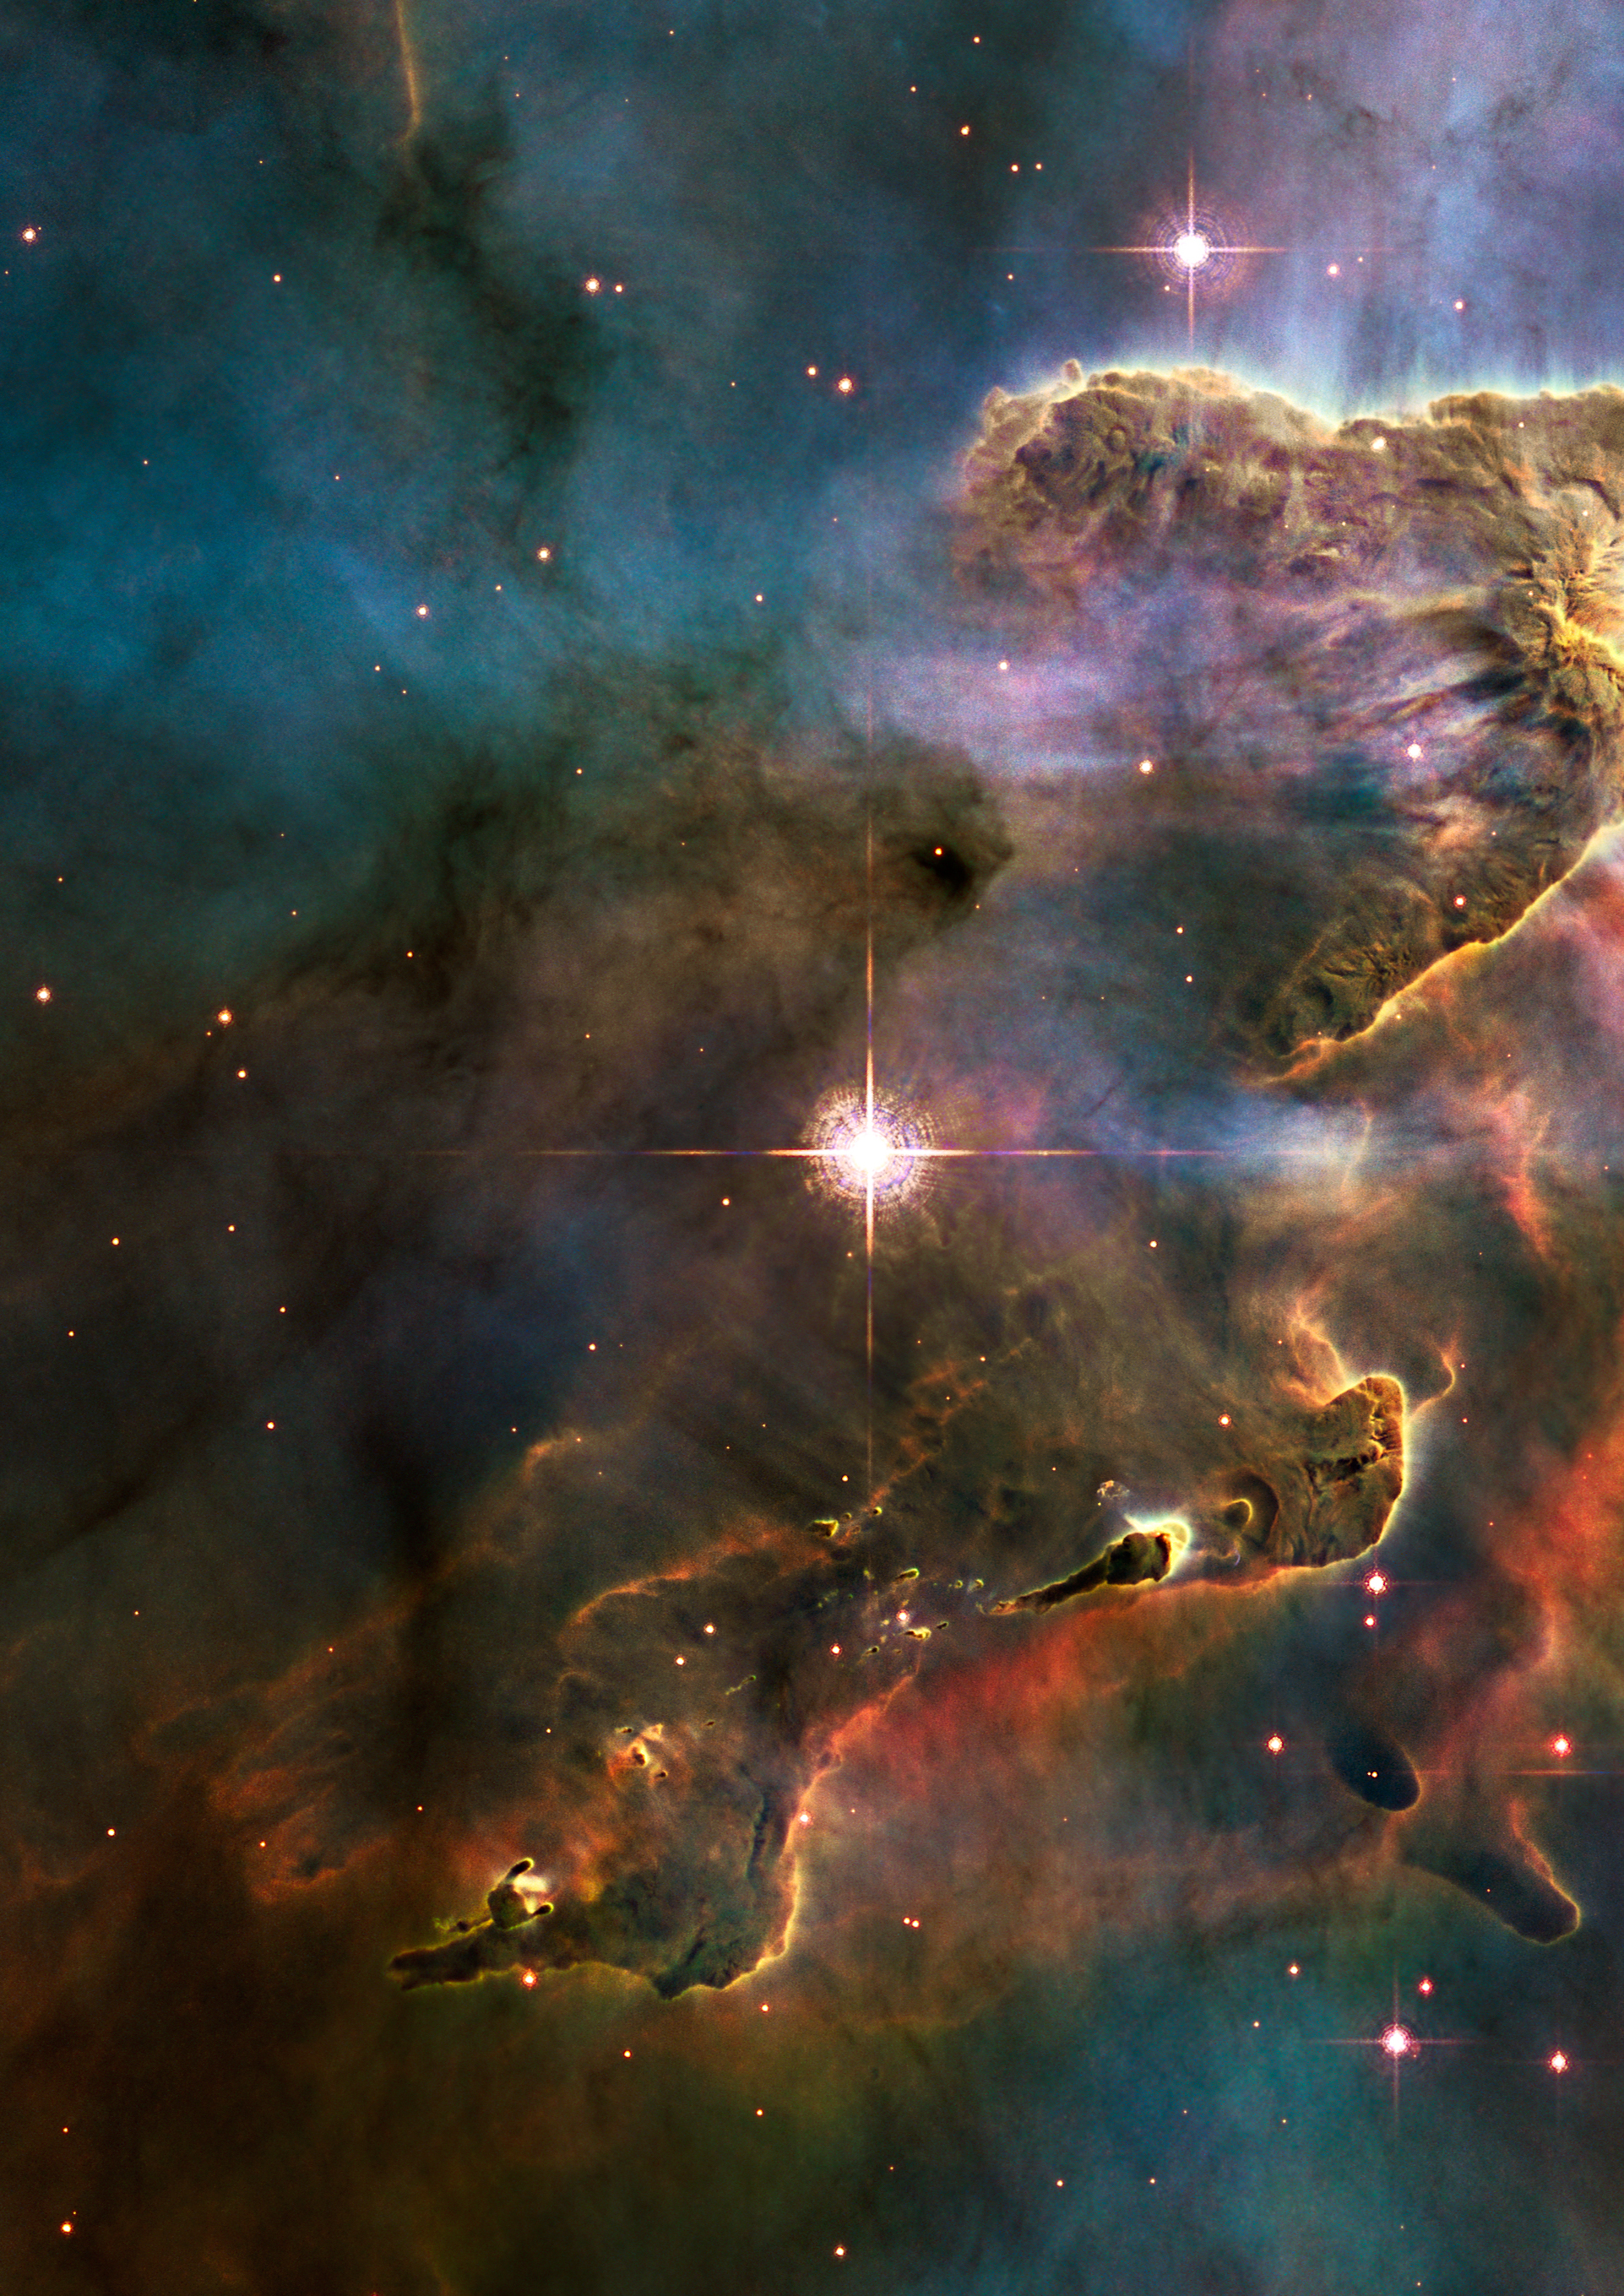
\includegraphics[width=\paperwidth]{Images/Carina_nebula_HST1}}
    }
    \BgThispage
    
    \fancyfoot[C]{\color{white}\thepage}
    \fancyfoot[L]{\vspace{3.5ex}\tiny\textcolor{white}{Credit: NASA, ESA, M. Livio, and the\\Hubble \nth{20} Anniversary Team (STScI)}}
    \clearpage
    \newpage
    
    \renewcommand{\CurrentTitleColor}{\color{white}}
\fi

\chapter{Introduction}
\label{ch:Introduction}

\ifsetDraft
\else
    \renewcommand{\CurrentTitleColor}{\color{black}}
    
%    \vspace*{\fill}
%    \setlength{\epigraphwidth}{0.85\textwidth}
%    {\color{white} \epigraph{\textit{Man muss noch Chaos in sich haben, um einen tanzenden Stern geb{\"a}ren zu k{\"o}nnen.}
%        \\
%        \vspace{2ex}
%        \textit{You must have chaos within yourself to give birth to a dancing star.}}{--- Friedrich Nietzsche, Also sprach Zarathustra (1883)}}
%    \vspace*{\fill}
    
    \backgroundsetup{
        scale=1,
        color=black,
        opacity=1,
        placement=top,
        angle=0,
        contents={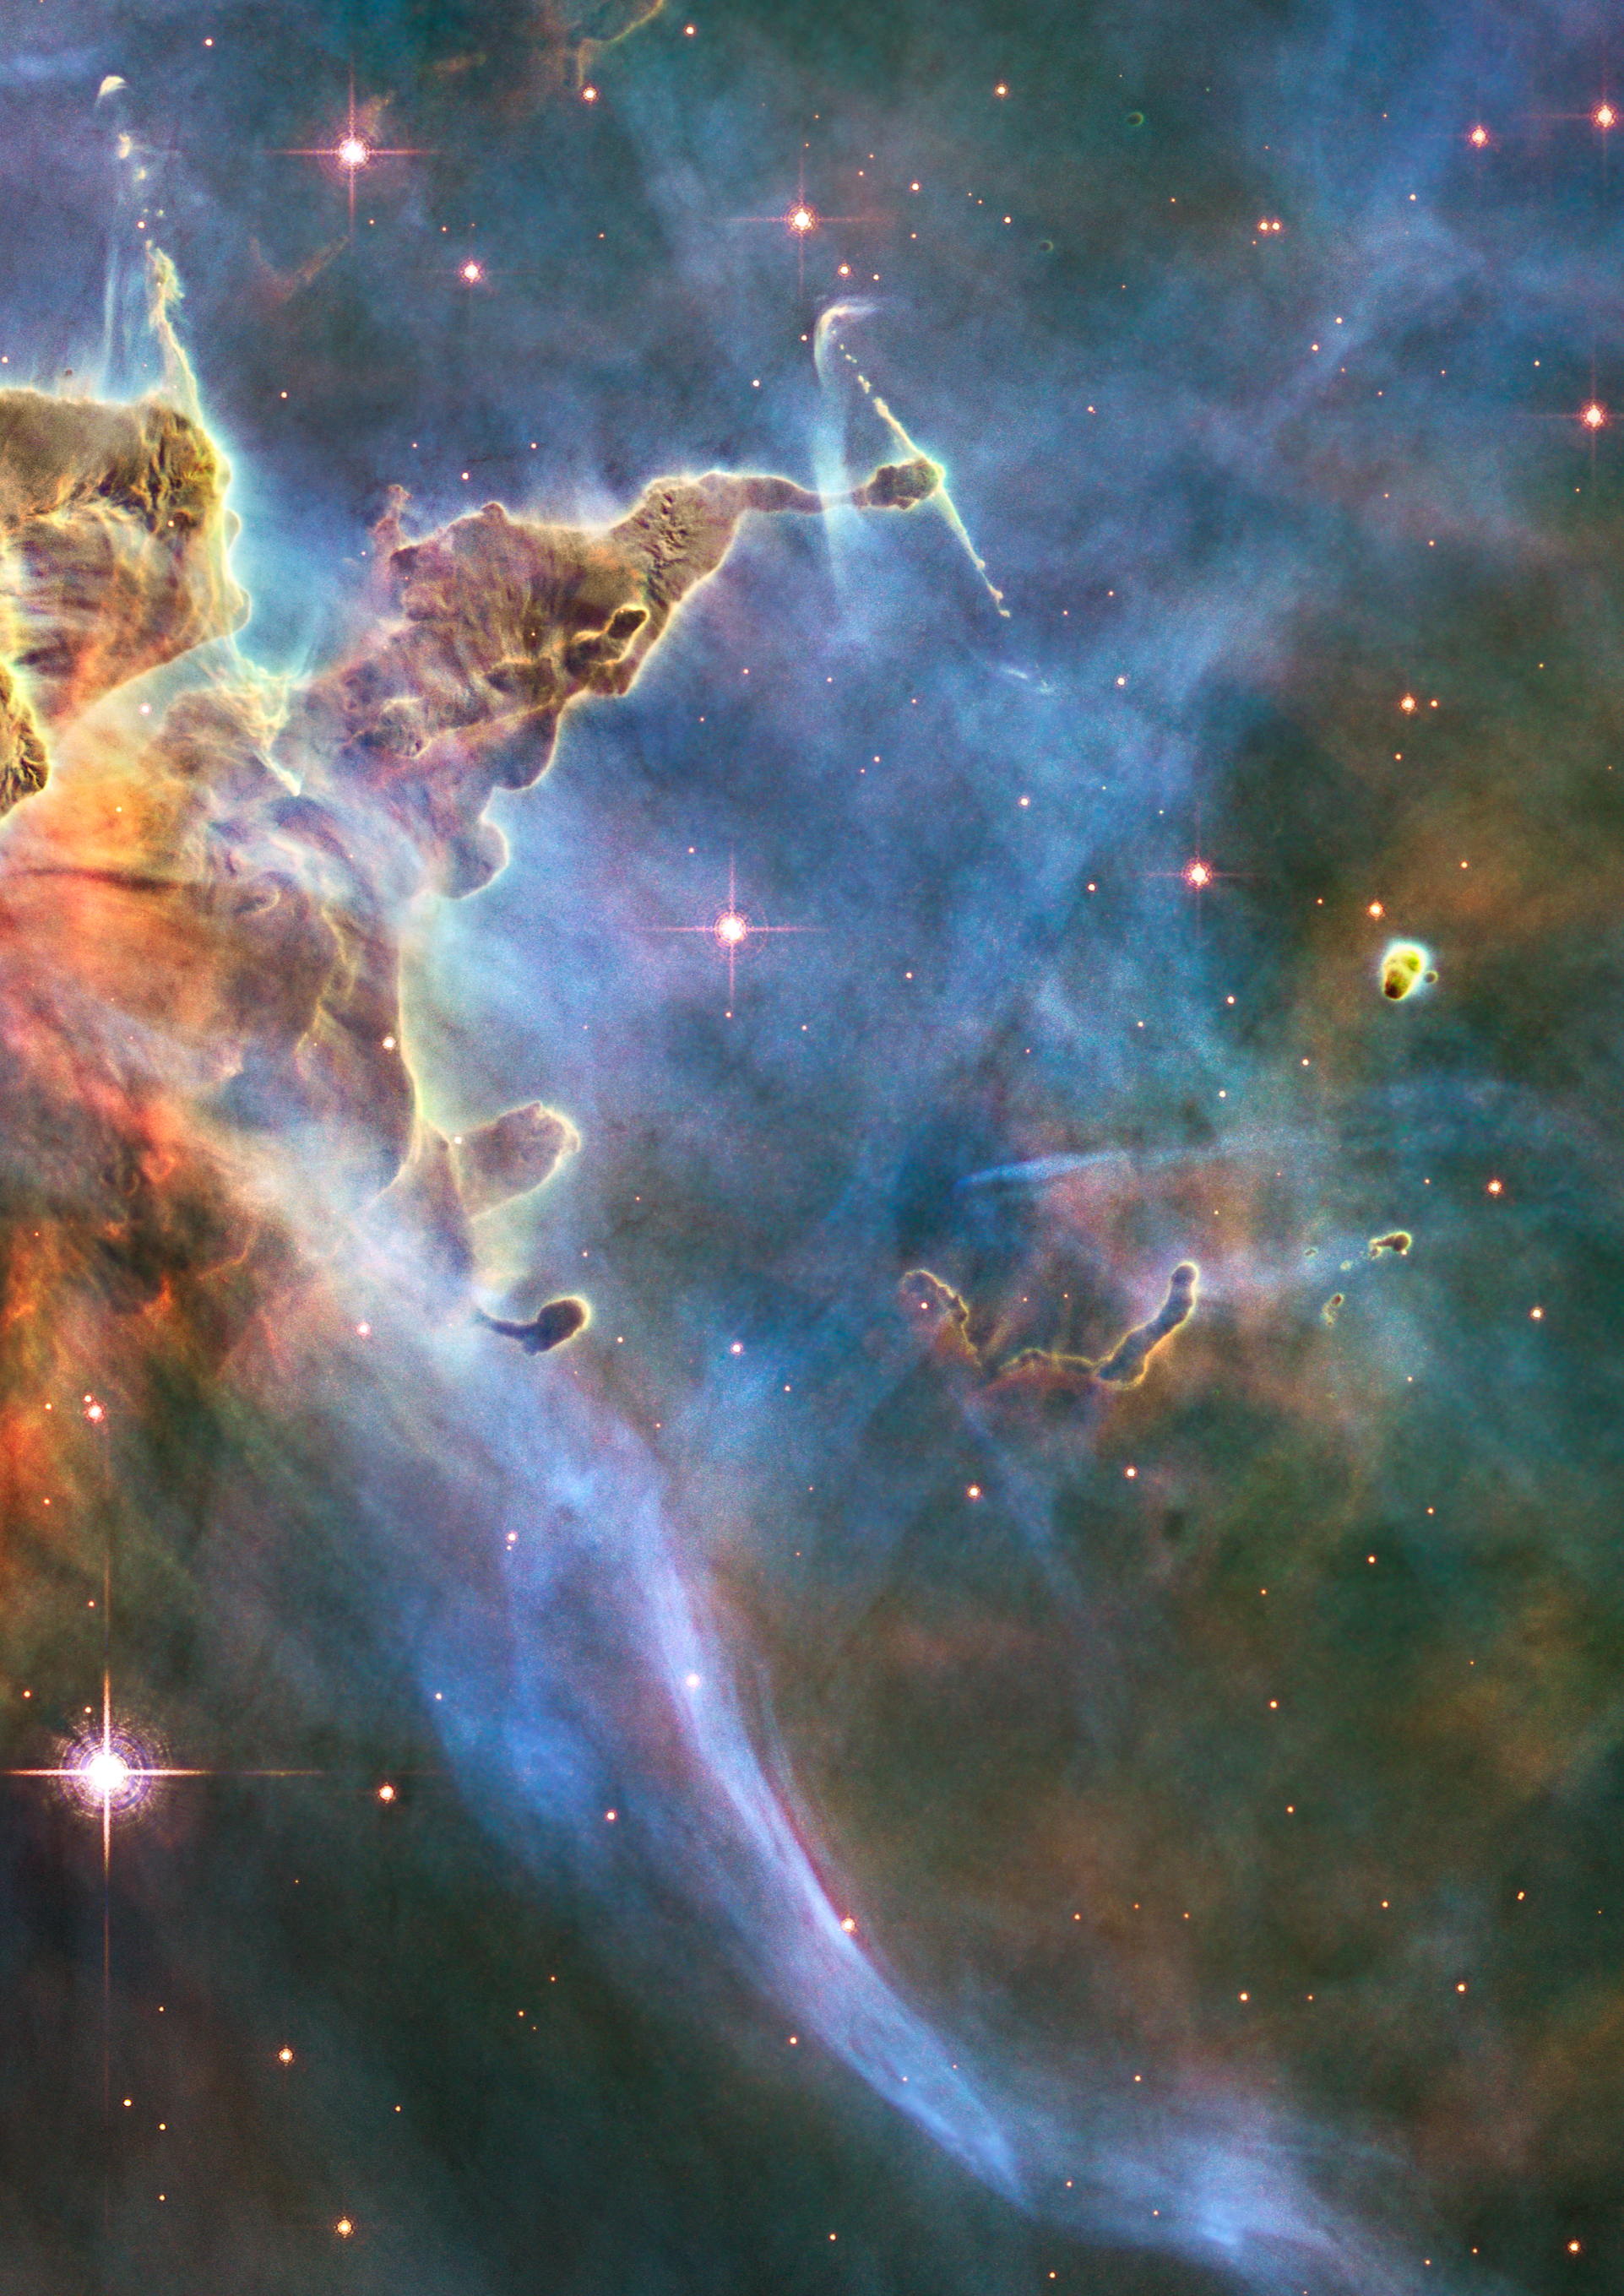
\includegraphics[width=\paperwidth]{Images/Carina_nebula_HST2}}
    }
    \BgThispage
    
    \fancyhf{}
    \fancyfoot[C]{\color{white}\thepage}
    \newpage
    \setFancyHdr
\fi

%\addcontentsline{toc}{chapter}{Introduction}
%\chaptermark{Introduction}{}

%\renewcommand\thefigure{I.\arabic{figure}}
%\setcounter{figure}{0}

\section{Cosmological background}

\lettrine{M}{ankind} has long marvelled at the complexity of the Universe. Technological developments have enabled a more detailed view of the complexity seen in the night sky than ever, as for example illustrated by \textit{JWST} in \cref{chIfig:SMACS}. However, humanity has sought to explain the origin and evolution of the Universe long before the invention of the telescope. Indeed, the formulation of several key principles that underpin our current understanding of the Universe can be traced back to ancient times. Pythagoras is believed to be the first to describe the Universe as \textgreek{κόσμος} (cosmos), ancient Greek for ``order'', emphasising his attempt to capture the seemingly chaotic Universe as an orderly system \citep[e.g.][]{1860Humboldt}. Subsequent advances in the field of \textit{cosmology} were, and still are, enabled by standing on the shoulders of giants. For instance, based on the work of \citet{Copernicus1543} and others -- initiating a considerable philosophical paradigm shift in cosmology that removed the Earth from the centre of the cosmos -- \citet{Newton1687} not only introduced novel mathematical techniques to describe the physical world, but also conceived an important cosmological notion with his law of \textit{universal} gravitation, asserting the law applied uniformly throughout space, laying important groundwork for the developments that would lead to the modern cosmological paradigm.
\begin{figure}
    \centering
    \includegraphics[width=\linewidth]{"Images/SMACS"}
    \caption[Colour composite image of the galaxy cluster SMACS 0723-73.]{Colour composite image of the galaxy cluster SMACS 0723-73, taken by \textit{JWST}/NIRCam (programme ID 2736, PI: Pontoppidan) as part of Early Release Observations \citep[EROs;][]{2022arXiv220713067P}, revealing a number of distant galaxies in the near-infrared (F444W in red, F356W in orange, F200W and F277W in green, F090W and F150W in blue). Credit: NASA, ESA, CSA, STScI.}
    \label{chIfig:SMACS}
\end{figure}

\subsection{Modern cosmology: theoretical and observational perspectives}
\label{chIssec:Modern_cosmology}

Founding the equivalence principle, \citet{1915SPAW.......844E} developed the theory of General Relativity (GR), relating the geometry of spacetime to the distribution of matter (or, equivalently, energy). However, it was realised soon after that GR can be applied as a theory of physical cosmology: a self-consistent mathematical description of the physical laws governing all matter across space and time, and indeed of the geometry of the spacetime continuum itself.\footnote{Note that a crucial assumption in these models is that the Universe is governed by the laws of GR: this implicitly assumes that gravity is the dominant force.} Modern cosmology is based on the \citeauthor{1915SPAW.......844E} field equation,
\begin{equation}
    \label{chIeq:Einstein_field_equation}
    R_{\mu \nu} - \frac{1}{2} g_{\mu \nu} R = \frac{8 \pi G}{c^4} T_{\mu \nu} \, ,
\end{equation}

\noindent where $R_{\mu \nu}$ is the Ricci tensor (defining the local curvature of spacetime), $g_{\mu \nu}$ is the metric (describing a local measure of time and distance), $R \equiv g^{\mu \nu} R_{\mu \nu}$ is the curvature scalar, $G$ is the gravitational constant, $c$ is the speed of light, and $T^{\mu \nu}$ is the energy-momentum tensor (encoding the matter content of the Universe).

\citet{1917SPAW.......142E} presented one of the first attempts at creating such a cosmological model within GR. Having realised that his theory only allowed for a contracting or expanding universe, Einstein introduced the concept of a cosmological constant $\Lambda$ (entering \cref{chIeq:Einstein_field_equation} as $\Lambda g_{\mu \nu}$) to contrive a static, but unstable, universe. Under the assumptions of homogeneity and isotropy collectively called the Cosmological Principle \citep{1933ZA......6....1M},\footnote{Equivalently, the Cosmological Principle states that the properties of the Universe appear the same to all observers; this is a generalisation of the Copernican Principle, which asserts that humans on Earth are not privileged observers.} a set of more general models of a universe governed by the laws of GR were independently constructed by \citet{1922ZPhy...10..377F} and \citet{1927PhDT.........6L}. These models describe a generic metric of curved spacetime containing a cosmological fluid with constant density $\rho$ and pressure $P$, which together form a solution to the field equations of GR.

Crucially, around the same time, it was found that in fact the Universe is not static, but expanding. Though many ``spiral nebulae'' had already been discovered \citep[e.g.][]{964AlSufi}, observations of Cepheid variables in these nebulae by \citet{1925ApJ....62..409H, 1926ApJ....63..236H} provided compelling evidence that they were themselves distant galaxies similar to the Milky Way, not diffuse gas clouds embedded within it. Then, \citet{1929PNAS...15..168H} reported that their recession velocity is proportional to their distance, $v = H_0 \, d$, an empirical relationship now known as Hubble's law. A uniformly expanding universe as predicted by the \citeauthor{1922ZPhy...10..377F} models provided an elegant explanation for this phenomenon. However, Einstein had not been alone in favouring the concept of a ``steady-state'' universe,\footnote{Famously, Einstein would later reportedly refer to the cosmological constant as ``the biggest blunder of my life''. Yet it may prove to be a fundamental constituent of our Universe, as will be discussed below.} since an expanding one brought about several uncomfortable ramifications. For instance, it implies that in the distant past, the Universe must have been increasingly denser and hotter, leading Fred Hoyle to scornfully coin the term \textit{Big Bang} for the hypothetical singularity at the beginning of time \citep[already discussed by][]{1927PhDT.........6L}.\footnote{In an interdepartmental feud, \citet{1961MNRAS.122..349R} would provide evidence that was considered the final nail in the coffin of the steady-state theory that Fred Hoyle advocated.}

\subsection{Interlude: observers in an expanding universe}
\label{chIssec:Observers_in_an_expanding_universe}

Because of the Cosmological Principle, all of the time dependence in the spatial component of the metric can be parametrised by $a(t)$, the \textit{scale factor} of the universe. Specifically,
\begin{equation}
    \label{chIeq:FLRW_metric}
    \dif s^2 = c^2 \dif t^2 - a^2(t) \left[ \frac{\dif r^2}{1 - Kr^2} + r^2 \left( \dif \theta^2 + \sin^2 \theta \dif \phi^2 \right) \right] \, ,
\end{equation}

\noindent with cosmic time $t$, spatial coordinates $(r, \theta, \phi)$, and $K \in \{ -1, 0, 1 \}$ parametrising the curvature ($K = 0$ corresponds to a ``flat'' universe). Under a coordinate transformation $\dif \chi = \dif r / \sqrt{1 - Kr^2}$, a light ray following a null geodesic ($\dif s^2 = 0$) travels through an expanding universe on a radial trajectory (i.e. $\dif \theta = \dif \phi = 0$) that obeys
\begin{equation}
    \label{chIeq:Null_geodesic}
    \frac{\dif \chi}{\dif t} = \pm \frac{c}{a(t)} \, ,
\end{equation}

\noindent where $\chi$ is interpreted as the \textit{comoving} (radial) geodesic distance. In a flat universe, the coordinate $r$ takes the role of the radial geodesic, $\chi = r$, but note this does not generalise for $K \neq 0$. The physical separation between two points along the radial trajectory at a fixed time $t$, measured via \cref{chIeq:FLRW_metric}, is $\Delta l = a(t) \Delta \chi$.

In general, a particle's comoving coordinates, $\vec{\chi} = \vec{x} / a(t)$ with $\vec{x}$ being its proper (i.e. physical) coordinates, are constant in time if it is at rest. The scale factor is typically normalised to $a(t_0) = a_0 = 1$ at the present day so that comoving and proper coordinates coincide.\footnote{All quantities with subscript $0$ will refer to their present-day value (i.e. at $t = t_0$).} It is further customary to define the Hubble parameter $H(t) = \dot{a}/a$ (where the dot indicates a time derivative), with present-day value $H(t_0) = H_0$, the Hubble constant. For historical reasons, it is often parametrised as $h \equiv H_0/(100 \, \mathrm{km \, s^{-1} \, Mpc^{-1}})$.\footnote{This dimensionless $h$ is not to be confused with the Planck constant.} To understand its connection with the findings of \citet{1929PNAS...15..168H}, we consider the velocity of an object at coordinates $\vec{x}$,
\begin{equation}
    \label{chIeq:Hubbles_law}
    \vec{v} = \frac{\dif \vec{x}}{\dif t} = \frac{\dif a}{\dif t} \, \vec{\chi} + a(t) \, \frac{\dif \vec{\chi}}{\dif t} = \frac{\dot{a}}{a} \, \vec{x} + \frac{\dif \vec{x}}{\dif t} = H \, \vec{x} + \vec{v}_\text{pec} \, ,
\end{equation}

\noindent where its \textit{peculiar velocity} is defined as $\vec{v}_\text{pec} = a(t) \, \dif \vec{\chi} / \dif t$. This can be interpreted as the excess velocity of an object, its movement on top of the Hubble flow, $\vec{v}_\text{H} = H \, \vec{x}$, which instead is the perceived movement purely due to the expansion of the universe. If the object is at rest, $\vec{v}_\text{pec} = 0$, so that \cref{chIeq:Hubbles_law} evaluated at $t = t_0$ recovers Hubble's law.

Without going into the details, it can be shown \citep[see e.g.][]{2010gfe..book.....M} that the field equations of GR in a homogeneous and isotropic universe translate into the \citeauthor{1922ZPhy...10..377F} equations:
\begin{align}
    \label{chIeq:Friedmann_equation1}
    H^2 & = \frac{8 \pi G}{3} \rho - \frac{K c^2}{a^2} + \frac{\Lambda c^2}{3} \, ,
    \\
    \label{chIeq:Friedmann_equation2}
    \frac{\ddot{a}}{a} & =  -\frac{4 \pi G}{3} \left( \rho + \frac{3 P}{c^2} \right) + \frac{\Lambda c^2}{3} \, ,
\end{align}

\noindent where $\Lambda$ is a cosmological constant, and $\rho$ and $P$ are the energy density and pressure of the cosmological fluid. The first law of thermodynamics (conservation of energy) within a volume $V$ requires
\begin{equation}
    \label{chIeq:First_law_thermodynamics}
    V \dif \rho + \left( \rho + \frac{P}{c^2} \right) \dif V = 0 \, ,
\end{equation}

\noindent so that given an equation of state $w \equiv P/\rho c^2$, the energy density $\rho_\text{x}$ of a specific type of matter evolves as
\begin{equation}
    \label{chIeq:Energy_density_scaling}
    \rho_\text{x} = \rho_{\text{x}, \, 0} \, \left( \frac{a}{a_0} \right)^{-3(1+w)} \, .
\end{equation}

Different types of energy content are characterised by the following equation of state: $w = 1/3$ for radiation or ultra-relativistic particles ($\rho_\text{r} \propto a^{-4}$; this implies the radiation temperature scales as $T_\text{r} \propto a^{-1}$, since $\rho_\text{r} \propto T_\text{r}^4$) and $w = 0$ for non-relativistic matter ($\rho_\text{m} \propto a^{-3}$). From \cref{chIeq:Friedmann_equation1,chIeq:Friedmann_equation2}, it can be seen even a cosmological constant can be described as having a (non-evolving) energy density $\rho_\Lambda =\Lambda c^2/8 \pi G$ and $w = -1$. The energy density in a universe containing a mixture of these can then be written as
\begin{equation}
    \label{chIeq:Total_energy_density}
    \rho = \rho_\text{r} + \rho_\text{m} + \rho_\Lambda = \frac{\rho_{\text{r}, \, 0}}{a^4} + \frac{\rho_{\text{m}, \, 0}}{a^3} + \rho_{\Lambda, \, 0} \, .
\end{equation}

From this equation, it follows that the early Universe ($a \ll 1$) was radiation-dominated (i.e. $\rho \approx \rho_\text{r}$), then became matter-dominated (with matter-radiation equality when $\rho_\text{r} = \rho_\text{m}$), and finally becomes $\Lambda$-dominated. Having incorporated the cosmological constant in the energy density, it makes sense to define a critical density,
\begin{equation}
    \label{chIeq:Critical_density}
    \rho_\text{crit} \equiv \frac{3 H^2(t)}{8 \pi G} \, ,
\end{equation}

\noindent which, according to \cref{chIeq:Friedmann_equation1}, is the density (including a contribution of $\Lambda$) at which the curvature disappears, $K = 0$. Further defining the density parameter, $\Omega_\text{x} = \rho_\text{x} / \rho_\text{crit}$, \cref{chIeq:Friedmann_equation1} can be rewritten as
\begin{align}
    \label{chIeq:Friedmann_equation1_alt1}
    H^2 & = \frac{8 \pi G}{3} \left( \frac{\rho_{\text{r}, \, 0}}{a^4} + \frac{\rho_{\text{m}, \, 0}}{a^3} + \rho_{\Lambda, \, 0} \right) - \frac{K c^2}{a^2} \nonumber
    \\
    & = H_0^2 \left( \frac{\rho_{\text{r}, \, 0}}{\rho_{\text{crit}, \, 0}} a^{-4} + \frac{\rho_{\text{m}, \, 0}}{\rho_{\text{crit}, \, 0}} a^{-3} + \frac{\rho_{\Lambda, \, 0}}{\rho_{\text{crit}, \, 0}} \right) - \frac{K c^2}{a^2} \nonumber
    \\
    & = H_0^2 \left( \Omega_{\text{r}, \, 0} a^{-4} + \Omega_{\text{m}, \, 0} a^{-3} + \Omega_{\Lambda, \, 0} \right) - \frac{K c^2}{a^2} \, ,
\end{align}

\noindent which specifies the evolution of the Hubble parameter in terms of the current-day density parameters, $\Omega_{\text{x}, \, 0} = \rho_{\text{x}, \, 0} / \rho_{\text{crit}, \, 0} = 8 \pi G \rho_{\text{x}, \, 0} / 3 H_0^2$. Alternatively, dividing \cref{chIeq:Friedmann_equation1} by $H^2$ gives
\begin{equation}
    \label{chIeq:Friedmann_equation1_alt2}
    1 - \Omega = 1 - \Omega_\text{r} - \Omega_\text{m} - \Omega_\Lambda = - \frac{K c^2}{H^2 a^2} \, ,
\end{equation}

\noindent from which again it can be seen that $\rho = \rho_\text{crit}$ (i.e. $\Omega = \Omega_\text{r} + \Omega_\text{m} + \Omega_\Lambda = 1$) for a flat universe. As will be discussed in \cref{chIssec:LCDM_model}, it turns out our Universe appears to have $\Omega_0 \approx 1$: it has no (or very little) curvature. In a flat universe dominated by energy content of one type of matter (e.g. a radiation-dominated universe), the scale factor evolves as
\begin{equation}
    \label{chIeq:Scale_factor}
    a(t) \propto t^\frac{2}{3(1+w)} \, .
\end{equation}

An important concept related to the scale factor is the \textit{cosmological redshift} seen by a present-day observer.\footnote{Doppler shift due to peculiar motion along the line of sight can add an additional kinematic blueshift or redshift.} It is defined by
\begin{equation}
    \label{chIeq:Redshift}
    1 + z = \frac{a_0}{a(t)} \, ,
\end{equation}

\noindent such that $z = 0$ corresponds to the present. In an expanding universe, light emitted by a distant source at an early time $t_\text{emit}$ is redshifted, $\lambda_\text{obs} = (1 + z) \, \lambda_\text{emit}$, since the universe has expanded by a factor of $a_0 / a(t_\text{emit}) = (1 + z)$ between emission and observation. Combined with the finite speed of light that allows astronomers to effectively look back in time, observing the distant Universe as it was in the past, cosmological redshift is an important (though not physical) measure of distance to faraway sources.

\subsection{Concordance cosmology: the \texorpdfstring{\LCDM}{ΛCDM} model}
\label{chIssec:LCDM_model}

Following several other observational breakthroughs, the so-called \LCDM\ model has been established over the past few decades as our standard cosmological model. Dynamical measurements testing gravity on the scales of galaxies and galaxy clusters \citep{1933AcHPh...6..110Z, 1973A&A....26..483R, 1974Natur.250..309E, 1974ApJ...193L...1O, 1978ApJ...225L.107R, 1980ApJ...238..471R} first hinted at the existence of a non-baryonic mass component exhibiting only gravitational interaction.\footnote{In cosmology, baryons are simply defined as ``visible'' matter (i.e. massive particles susceptible to electromagnetic interactions); unlike in particle physics, this includes leptons.} \textit{Dark matter}, now hypothesised to be made up of a massive, weakly interacting particle, gradually became an accepted paradigm. The study of distant supernova (SN) explosions furthermore led to the discovery of the accelerated expansion of the Universe \citep{1998AJ....116.1009R, 1998ApJ...507...46S, 1999ApJ...517..565P}, indicating the additional presence of \textit{dark energy}. As a more general version of Einstein's cosmological constant, dark energy causes spacetime to expand, which counteracts (and at the present epoch, even outweighs) gravitational contraction of the Universe.

The \LCDM\ model is thus named after these two main constituents: dark energy (specifically behaving like a cosmological constant $\Lambda$, i.e. $w = -1$) and cold dark matter (CDM).\footnote{The coldness refers to the thermal motions of the dark matter particles when they decouple, as will be discussed in \cref{chIsssec:Dark_matter_instabilities}.} The discovery of the cosmic microwave background (CMB) radiation \citep{1965ApJ...142..419P, 1965ApJ...142..414D} allowed access to another powerful observational probe of cosmology, which has since firmly anchored the \LCDM\ paradigm.

First of all, the CMB provides strong evidence for the Big Bang theory as it nearly perfectly resembles blackbody emission (cf. \cref{chIssec:Effects_of_dust}), observed today at $T_{\text{CMB}, \, 0} = 2.725 \, \mathrm{K}$ \citep[e.g.][]{2009ApJ...707..916F}, proving the early Universe was hot and dense \citep[in fact, the existence of the CMB in a Big Bang model had been predicted before its discovery;][]{1949RvMP...21..367G}. After this hot, ionised plasma in the early Universe had cooled down sufficiently due to expansion, protons and electrons were able to recombine \citep[at a redshift of $z \sim \num{1100}$; e.g.][]{1985A&A...149..144J}.\footnote{Note that this terminology is misleading, since the epoch of recombination was the very first time that stable, neutral atoms were able to form.} The sudden phase transition turned the hot plasma into neutral gas that was no longer opaque, releasing the (henceforth) ever-present relic radiation. Furthermore, the extremely high degree of isotropy seen in the CMB, with fluctuations of the order of $\delta T / T \sim 10^{-5}$, makes a compelling case for the validity of the Cosmological Principle, while the angular power spectrum of precisely these fluctuations is described remarkably well by \LCDM\ \citep{2020A&A...641A...1P}. Detailed fitting procedures provide high-precision measurements of its six free parameters. The latest results \citep[e.g.][]{2020A&A...641A...6P} show that:
\begin{enumerate}[label=(\roman*)]
    \item the current expansion rate of the Universe, as measured through the Hubble constant, is $H_0 = 67.4 \pm 0.5 \, \mathrm{km \, s^{-1} \, Mpc^{-1}}$;
    \item dark matter significantly dominates over baryonic matter, which only makes up around one sixth of the matter content ($\Omega_{\text{b}, \, 0} \sim 0.05$, while $\Omega_{\text{m}, \, 0} \sim 0.3$);
    \item dark energy currently trumps matter ($\Omega_{\Lambda, \, 0} \sim 0.7$) and is consistent with a cosmological constant (i.e. equation of state $w = -1$);
    \item the total density appears to be close to the critical density ($\Omega_0 = 1$), which implies the Universe is spatially flat.
\end{enumerate}

Unless explicitly mentioned otherwise (in particular in \cref{ch:Prospects_for_observing_the_low-density_cosmic_web_in_Lya_emission}), we assume $\Omega_{\text{m}, \, 0} = 0.3$, $\Omega_{\Lambda, \, 0} = 0.7$, and $H_0 = 70 \, \mathrm{km \, s^{-1} \, Mpc^{-1}}$ (i.e. $h = 0.7$) throughout.

\subsection{Structure formation in a homogeneous and isotropic universe}
\label{chIssec:Structure_formation_in_a_homogeneous_and_isotropic_universe}

Despite the success of the \LCDM\ model in reproducing the statistical properties of the CMB, several conceptual problems remain. How can a homogeneous and isotropic model universe, adhering to the assumptions of the Cosmological Principle, ever achieve the observed complexity such as that shown in \cref{chIfig:SMACS}? This issue can be resolved by considering the model as an approximation that becomes valid at sufficiently large scales \citep[$l \gtrsim 200 \, \mathrm{cMpc}$ according to simulations, where $\mathrm{cMpc}$ denotes a comoving megaparsec; e.g.][]{2010MNRAS.405.2009Y}. Indeed, a strictly homogeneous universe would not see the formation of any structure; such a model universe devoid of galaxies, stars, and planets is evidently not a representative model for the observed Universe. This statement may seem obvious, but it underlines the effectiveness of the relatively simple \LCDM\ model at explaining the formation of complex cosmological structures as local deviations from a homogeneous background.

Another challenge facing the \LCDM\ model, then, are the initial conditions, which need to be understood in order to make useful predictions about the cosmic structure observed today. As first shown by \citet{1970PhRvD...1.2726H} and \citet{1972MNRAS.160P...1Z}, galaxy-sized structures can be formed by ``primordial'' fluctuations (i.e. perturbations that are in place at very early times) only if these take the form of a scale-invariant power spectrum. Things, however, become problematic at very early times, particularly when typical scales in the universe approached the Planck scale ($t_\text{P} \sim 10^{-43} \, \mathrm{s}$ and $m_\text{P} \sim 10^{19} \, \mathrm{GeV}/c^2$). On larger scales, gravity is assumed to dominate over the electromagnetic, strong, and weak interactions but at sufficiently small scales these forces start to compete with gravity, requiring a theory of quantum gravity to be properly understood.\footnote{A quantum description of matter does not have a definitive spatial distribution (let alone true homogeneity), which makes a reconciliation of quantum theory and GR difficult.} Certainly, in the so-called Planck epoch -- the first $t_\text{P} \sim 10^{-43} \, \mathrm{s}$ after the Big Bang -- the basic \LCDM\ model is no longer valid. Further problems arise from interpreting observations of the CMB: its isotropy suggests polar-opposite regions, despite not having been in causal contact, were somehow at (nearly perfect) thermal equilibrium when the CMB was released \citep[the ``horizon problem'';][]{1968ApJ...151..431M}. Moreover, the spatial flatness observed today requires extreme fine-tuning of the initial curvature of the Universe \citep[the ``flatness problem'';][]{1979grec.conf..504D}.

It turns out that a solution for the latter two problems, namely extending the \LCDM\ model with a brief period of exponential expansion (\textit{inflation}) shortly after the Big Bang, also alleviates the issue of not (yet) having a unifying theory valid at extremely high energies \citep{1980PhLB...91...99S, 1980ApJ...241L..59K, 1981PhRvD..23..347G, 1982PhLB..108..389L, 1982PhRvL..48.1220A}. Without having to specify the exact physical properties of the Universe at the Planck epoch, the quantum fluctuations of the scalar field driving inflation (with corresponding particle called the \textit{inflaton}) simultaneously provide a natural explanation for a nearly scale-invariant Gaussian random field of initial density perturbations \citep{1982PhLB..115..295H, 1982PhRvL..49.1110G, 1983PhRvD..28..679B}.

Although several modifications and/or replacements have been proposed,\footnote{There exists observational evidence that further extensions of the \LCDM\ model may be required. There are, for instance, hints of cosmic anisotropy \citep[e.g.][]{2022arXiv220805018P} and the Hubble constant determined from the CMB, $H_0 = (67.4 \pm 0.5) \, \mathrm{km \, s^{-1}  \, Mpc^{-1}}$, deviates from local measurements \citep{2020A&A...641A...6P}. Other tension, such as the ``cusp-core'' and ``missing-satellite'' problems are generally attributed to the detailed effects of galaxy formation \citep[``baryonic physics''; e.g.][]{2012MNRAS.421.3464P, 2016ApJ...827L..23W}.} the \LCDM\ model (coupled to inflation) is unrivalled in its ability to accurately explain and quantitatively reproduce a plethora of statistical properties of observed cosmic structure. It explains the formation and evolution of structure seen across more than $\ssim 99.997\%$ of cosmic time: from the CMB to the abundance of galaxies observed today. The next section will go into the details of the formation and evolution of these galaxies in a \LCDM\ universe.

\section{Galaxy formation and evolution: a brief history of time}

In the \LCDM\ model, structures of visible matter, such as galaxies, form in hierarchical manner on top of a dark matter firmament, all having grown from inflated quantum fluctuations. The following sections will discuss the various assembly stages of these structures (as well as their enrichment with heavy elements), shown schematically in \cref{chIfig:Cosmic_timeline} as a timeline of the Universe. Shortly after the Big Bang, inflation sets the initial conditions for the formation of structure, which can be probed via the CMB (discussed in \cref{chIssec:Inflation_until_CMB}). Density fluctuations grow throughout the dark ages (\cref{chIssec:Growt_of_structure_in_the_linear_regime,chIssec:Non-linear_collapse}), resulting in the formation of the first stars and galaxies at cosmic dawn (\cref{chIssec:Galaxy_formation}). The onset of star formation (\cref{chIssec:Star_formation_and_stellar_evolution}), in turn, initiated the creation of the first heavy elements (\cref{chIssec:Chemical_enrichment}) and led to the reionisation of the Universe (\cref{chIssec:Epoch_of_Reionisation}). However, all good things come to an end and at present, we find ourselves in an epoch of declining star formation activity (\cref{chIssec:Cosmic_noon_and_the_epoch_of_quenching}).
\begin{figure}
    \centering
    \includegraphics[width=\linewidth]{"Images/NAOJ_timeline_highres"}
    \caption[Schematic timeline of the Universe.]{Schematic timeline of the Universe. Time increases from left to right, is indicated on top, redshift as defined in \cref{chIeq:Redshift} increases from right to left on the bottom (note the scales are not linear). Several important evolutionary stages of the early Universe are indicated, focusing on Cosmic Reionisation (\cref{chIssec:Epoch_of_Reionisation}). Credit: NAOJ.}
    \label{chIfig:Cosmic_timeline}
\end{figure}

\subsection{Inflation until the CMB: synthesis of the first elements}
\label{chIssec:Inflation_until_CMB}

Towards the end of inflation, the release of the potential energy of the inflaton field (\textit{reheating}) leaves the Universe in a hot and dense state \citep[ultimately the source of the blackbody nature of the CMB;][]{1994PhRvL..73.3195K}. Quantum fluctuations of the inflaton field cause a (nearly) scale-invariant Gaussian random field of density perturbations to be imprinted on the density field, as described above. Within a fraction of a second after the Big Bang, the Universe expands and cools down sufficiently to enter the realm of the Standard Model of particle physics ($T \lesssim 10^{15} \, \mathrm{K}$ or $E \lesssim 150 \, \mathrm{GeV}$) and is now filled with a quark-gluon plasma. Still within the first second of cosmic time, quarks are able to settle into hadrons, including protons and neutrons.

Importantly, interactions between protons and neutrons began to allow atomic nuclei heavier than hydrogen (i.e. a proton) to form in a process called Big Bang Nucleosynthesis \citep[BBN; work on this was pioneered by][]{1949RvMP...21..367G}. However, requiring a temperature that is low compared to the binding energy of a nucleus means that the density was no longer high enough for (a sufficiently high interaction rate of) many-body collisions, so that only the lightest elements (He, Li) can form at appreciable abundances \citep{1967ApJ...148....3W}.\footnote{The chemical network of two-body reactions is not able to go beyond lithium due to a lack of stable nuclei with atomic weight of 5 or 8 \citep[e.g.][]{2010gfe..book.....M}. The origin of heavier elements will be discussed in \cref{chIssec:Chemical_enrichment}.} As a result, primordial nucleosynthesis is predicted to yield a $\ssim 25\%$ mass fraction of helium, in excellent agreement with observations \citep[and hence considered a key validation of the Big Bang theory;][]{2016RvMP...88a5004C}.

As the Universe expands and cools down further, species start to \textit{decouple} from the primordial plasma, meaning they fall out of thermal equilibrium. At $z \sim 3400$, the energy densities of relativistic particles (radiation) and matter become equal and the Universe enters the matter-dominated phase. As discussed above, CMB photons are released as matter and radiation decouple at $z_\text{dec} \sim 1100$, or about $\num{380000} \, \mathrm{yr}$ after the Big Bang \citep{2010gfe..book.....M}. This signified the beginning of the cosmic \textit{dark ages} (see \cref{chIfig:Cosmic_timeline}).

\subsection{Growth of structure in the linear regime}
\label{chIssec:Growt_of_structure_in_the_linear_regime}

Ironically, radiation freely roamed the Universe for the first time during the dark ages, but they would have been truly dark to the human eye: CMB photons were redshifting away from visible wavelengths while there were no other optical light sources (causing the dark ages to appear rather uninteresting in \cref{chIfig:Cosmic_timeline}). Directly observing the dark ages, however, may in theory be achieved through the 21-cm line emitted by neutral hydrogen \citep[e.g.][]{2006PhR...433..181F}. Furthermore, like their historical counterpart, the fact that there is no clear record of what exactly happened does not make the dark ages any less eventful: primordial density fluctuations would steadily grow -- in fact, enhanced dark matter perturbations were already in place, as will be discussed in \cref{chIsssec:Dark_matter_instabilities} -- which would soon lead to the formation of the astrophysical objects.

As first shown by \citet{1902RSPTA.199....1J}, gravitational instability allows perturbations to grow into evolved structures provided their size exceeds a critical threshold, below which internal pressure prevents collapse. The \citeauthor{1902RSPTA.199....1J} formalism considers the linear regime of perturbations in the density field $\rho$, $\delta \equiv (\rho - \bar{\rho}) / \bar{\rho}$ with $\delta \ll 1$, against a background of constant density, $\bar{\rho}$. In the Newtonian description of a non-relativistic fluid in an expanding universe, the perturbations, decomposed the into Fourier modes (with comoving wavenumber $k = 2\pi a(t) / \lambda$), can be shown to satisfy
\begin{equation}
    \label{chIeq:Jeans_instability}
    \ddot{\delta}_k + 2 H \dot{\delta}_k + \left( \frac{c_\text{s}^2 k^2}{a^2} - 4 \pi G \bar{\rho} \right) \delta_k = 0 \, ,
\end{equation}

\noindent where $c_\text{s}$ is the adiabatic speed of sound. This describes a damped harmonic oscillator with angular frequency $\omega_k$ satisfying $\omega_k^2 = \frac{c_\text{s}^2 k^2}{a^2} - 4 \pi G \bar{\rho}$. The \citeauthor{1902RSPTA.199....1J} length, a critical scale for which $\omega_k^2 = 0$, is given in proper units by
\begin{equation}
    \label{chIeq:Jeans_length}
    \lambda_\text{J} = c_\text{s} \sqrt{\frac{\pi}{G \bar{\rho}}} \, ,
\end{equation}

\noindent with corresponding \citeauthor{1902RSPTA.199....1J} mass enclosed by a sphere of diameter $\lambda_\text{J}$,
\begin{equation}
    \label{chIeq:Jeans_mass}
    M_\text{J} = \frac{4}{3} \pi \bar{\rho} \left( \frac{\lambda_\text{J}}{2} \right)^3 = \frac{\pi}{6} \bar{\rho} \lambda_\text{J}^3 \, .
\end{equation}

Modes below the critical scale, $\lambda \ll \lambda_\text{J}$, act as acoustic waves, oscillating around hydrostatic equilibrium where pressure counteracts gravity. On the other hand, gravity is able to overcome the internal pressure support for perturbations satisfying the criterion for collapse, $\lambda \gg \lambda_\text{J}$. In this case, $\omega_k$ is imaginary and the equation describes a (stationary) growing or decaying mode instead. In both cases, the universe's expansion offers additional support against gravitational collapse -- the ``Hubble drag'' -- causing a damping of the acoustic waves and a slowing in the growth (or decay) of an instability.

\subsubsection{Baryonic instabilities}
\label{chIsssec:Baryonic_instabilities}

When radiation and baryons are still coupled, radiation pressure is sufficiently high to prevent the collapse of all but the largest structures, corresponding to $M_\text{J} \sim 10^{16} \, \mathrm{M_\odot}$ \citep[the mass of the largest galaxy clusters;][]{2010gfe..book.....M}. Formally, the \citeauthor{1902RSPTA.199....1J} analysis needs be extended to include relativistic effects \citep[e.g.][]{1946ZhETF..16..587L} as the assumption of a non-relativistic background fluid no longer holds in the radiation-dominated phase, but the result is qualitatively the same. As a consequence, perturbations of the photon-baryon plasma in the pre-recombination era drive baryon acoustic oscillations (BAO), whose imprint can be seen in the CMB.

Another consequence of relativistic effects is a distinction between the growth of modes within and beyond than the (comoving) particle horizon at a given time $t$,
\begin{equation}
    \label{chIeq:Particle_horizon}
    \chi_\text{h}(t) = \int_{0}^{t} \frac{c \dif t'}{a(t')} \, ,
\end{equation}

\noindent which is interpreted as the radius beyond which light rays information cannot have reached the origin (cf. \cref{chIeq:Null_geodesic}). It increases with time, at least in the radiation- and matter-dominated eras; modes therefore only start to grow once they have entered the horizon, while super-horizon modes are ``frozen''. Before recombination, all sub-horizon modes of baryonic perturbations fall below the \citeauthor{1902RSPTA.199....1J} scale so that each mode entering the horizon assumes oscillatory behaviour \citep[e.g.][]{1981ApJ...248..885P}.

Recombination then marks a sharp phase transition where free electrons were rapidly captured, although this was not quite an instantaneous process. There was a brief period where the mean free path (MFP) of photons was some finite value, in contrast to the earlier radiation-dominated phase and the later dark ages where, relative to scales $\lambda_\text{g}$ relevant for galaxy formation, the MFP was effectively zero ($\lambda_\text{MFP} \ll \lambda_\text{g}$) and infinity ($\lambda_\text{MFP} \gg \lambda_\text{g}$), respectively \citep{1968ApJ...151..459S}. As a result, photons preferentially diffuse from overdense into underdense regions, the so-called \citeauthor{1968ApJ...151..459S} damping, thereby smoothing out small-scale perturbations below the damping scale of $M_\text{d} \sim 10^{14} \, \mathrm{M_\odot}$. Considering baryonic fluctuations alone therefore suggests galaxy formation occurs in a top-down scenario, requiring the surviving large perturbations to fragment into smaller, galaxy-sized ($M \sim 10^{11} \, \mathrm{M_\odot}$) structures (in disagreement with observations).

After decoupling, radiative pressure support falls away and is replaced by gas pressure. At this stage, baryons can be described well by an ideal, non-relativistic, monoatomic gas at temperature $T$, so that
\begin{equation}
    \label{chIeq:Ideal_gas}
    c_\text{s} = \frac{5}{3} \frac{k_\text{B} T}{m_\text{p}} \, ,
\end{equation}

\noindent where $k_\text{B}$ is the Boltzmann constant and $m_\text{p}$ is the proton mass. This results in a much-reduced \citeauthor{1902RSPTA.199....1J} mass approximately equal to the size of a globular cluster, $M_\text{J} \sim 10^{6} \, \mathrm{M_\odot}$, suggesting structure on galactic scales start to collapse at this point \citep{2010gfe..book.....M}. Indeed, it can be shown that for a pressureless fluid (or equivalently for sufficiently large modes, $\lambda \gg \lambda_\text{J}$) the growing mode in the matter-dominated regime scales (almost) linearly with the scale factor, $\delta \appropto a \propto (1+z)^{-1}$ \citep{1992ARA&A..30..499C}.
\begin{figure}
    \centering
    \includegraphics[width=\linewidth]{"Figs/Neutral_gas_distribution"}
    \caption[Simulated column density of neutral hydrogen at $z=4.8$.]{Simulated column density of neutral hydrogen, $N_\text{\ion{H}{I}}$, in a simulation snapshot at $z = 7$ (cf. \cref{ch:Prospects_for_observing_the_low-density_cosmic_web_in_Lya_emission}). The neutral hydrogen distribution is shown for the full extent of the simulation box, $40 \times 40 \, h^{-2} \, \mathrm{cMpc}^2$, for a $\ssim 5.5 \, h^{-1} \, \mathrm{cMpc}$ depth. Baryonic matter closely follows the underlying dark matter distribution, without which fluctuations seen in the CMB could not have grown into the structures observed today (as discussed in \cref{chIsssec:Baryonic_instabilities,chIsssec:Dark_matter_instabilities}). The cosmological density field (here traced via neutral hydrogen) reveals a complex, web-like structure with large voids and overdense regions.}
    \label{chIfig:Neutral_gas_distribution}
\end{figure}

The relatively slow growth rate combined with the effect of \citeauthor{1968ApJ...151..459S} damping, however, requires large initial fluctuations to form observed clusters of galaxies (with masses comparable to the damping scale, $M \gtrsim 10^{14} \, \mathrm{M_\odot}$). If these structures are seeded by initial perturbations in the baryonic density field, and the onset of growth occurs at decoupling, $z_\text{dec} \sim 1100$, the observed temperature fluctuations in the CMB\footnote{Perturbations in the radiation temperature, $\delta T$, are related to those in matter density, $\delta$, as $\delta T / T = \delta/3$, since $T_\text{r} \propto \rho_\text{m}^{1/3}$ (this can be seen from the scaling relations $T_\text{r} \propto a^{-1}$ and $\rho_\text{m} \propto a^{-3}$).} would need to be of the order of $\delta T / T \sim 10^{-3}$ to reach $\delta \sim 1$ (where non-linear structure forms; \cref{chIssec:Non-linear_collapse}) at $z = 0$, two orders of magnitude larger than what is observed. The severe mismatch between purely baryonic cosmological models of galaxy formation and the observed Universe provides further key evidence for the existence of a significant dark matter component, which can remedy these issues.

\subsubsection{Dark matter instabilities}
\label{chIsssec:Dark_matter_instabilities}

Dark-matter perturbations undergo a substantially different evolution compared to the baryonic behaviour discussed above, since dark matter had decoupled at very early times owing to its weak electromagnetic interaction. In the radiation-dominated regime, dark matter (sub-horizon) perturbations can already slowly grow, scaling logarithmically with the scale factor.\footnote{With the exception that for prevailing non-relativistic perturbations in a background density dominated by a relativistic component (i.e. $\bar{\rho}_\text{r} \delta_\text{r} \ll \bar{\rho}_\text{dm} \delta_\text{dm}$ in the radiation-dominated phase), as is the case for dark matter perturbations approaching the time of matter-radiation equality, the growing mode actually stagnates due to the Hubble drag \citep{1974A&A....37..225M}.}

Most importantly, however, the dark matter instabilities start to grow at near-linear pace from the matter-radiation equality onwards \citep{1992ARA&A..30..499C}, allowing them to get ahead of the baryonic perturbations that are trapped in acoustic waves until recombination. With the radiation field having been critically diluted after the matter-radiation equality, dark matter effectively becomes the Universe's main constituent, while baryons only serve a subdominant role making up one sixth of the matter content (\cref{chIssec:LCDM_model}). After recombination, baryons therefore quickly fall into the strong gravitational potential wells of dark matter overdensities, circumventing the effects of \citeauthor{1968ApJ...151..459S} damping by which dark matter is not affected, since it had decoupled long before recombination.

However, dark matter still suffers from the effect of \textit{free streaming}: initial velocities, imposed by thermal equilibrium in the primordial plasma, also have a smoothing effect on small-scale density enhancements. Equivalently, the \citeauthor{1902RSPTA.199....1J} formalism can still be applied to the collisionless dark matter if the adiabatic speed of sound $c_\text{s}$ in \cref{chIeq:Jeans_length} is replaced by its velocity dispersion $\sigma_\text{dm}$, which acts effectively as a pressure on small scales. Less massive dark matter particles have higher velocities when they decouple, which washes out small-scale density perturbations. A characteristic particle mass of $m_\text{g} \sim 1 \, \mathrm{keV}/c^2$ leads to perturbations being affected at (and below) typical galactic scales, making the case for CDM ($m \ll m_\text{g}$) as opposed to warm ($m \sim m_\text{g}$) or hot ($m \gg m_\text{g}$) dark matter cosmologies \citep[e.g.][]{1982ApJ...263L...1P}.

To illustrate the growth of structure in the ($\Lambda$)CDM paradigm, the simulated neutral hydrogen column density, $N_\text{\ion{H}{I}}$,\footnote{Here, \ion{H}{I} is the spectroscopic notation for neutral hydrogen; see \cref{chIssec:Definitions_and_notation} for details.} of a large cosmological volume at $z = 7$ is shown in \cref{chIfig:Neutral_gas_distribution}. The specific cosmological simulation used to produce this neutral hydrogen distribution will be described in detail in \cref{ch:Prospects_for_observing_the_low-density_cosmic_web_in_Lya_emission} (see \cref{appPfig:NHI} in particular). The displayed area is equal to the full simulation box extent, $40 \times 40 \, h^{-2} \, \mathrm{cMpc}^2$, over a depth of $\ssim 5.5 \, h^{-1} \, \mathrm{cMpc}$ (that would correspond to a \lymana\ narrowband image with $\Delta \lambda_\text{obs} = 17.5 \, \Angstrom$; cf. \cref{chPsssec:Narrowband}). The cosmological density field, here traced via neutral hydrogen, reveals a complex, web-like structure called the \textit{cosmic web} at scales above approximately a few $\mathrm{cMpc}$ (though it starts to appear homogeneous at $l \gg 200 \, \mathrm{cMpc}$, as discussed in \cref{chIssec:Structure_formation_in_a_homogeneous_and_isotropic_universe}; see also \cref{ch:Prospects_for_observing_the_low-density_cosmic_web_in_Lya_emission}).

The precise appearance of the cosmic web is a result of the hierarchical formation of structure: small structures form first, merging into increasingly larger objects. Though directly observing the cosmic web is extremely challenging, since the bulk of baryonic matter hardly emits any light, efforts are underway to do precisely this, as will be discussed in \cref{ch:Prospects_for_observing_the_low-density_cosmic_web_in_Lya_emission}. The density field can be probed indirectly, however, via the large-scale distribution of galaxies, with the $\Lambda$CDM model predicting each galaxy is placed at the centre of a \textit{dark matter halo}. To understand the next stages in the process of galaxy formation, taking place at scales orders of magnitude smaller than that of the cosmic web shown in \cref{chIfig:Neutral_gas_distribution}, linear theory does not suffice any more: once $\delta \sim 1$, non-linear effects start to play a role as the perturbation itself becomes more important than the background density. Overdense regions then decouple from the Hubble flow and (in the case of dark matter) establish a dynamical quasi-equilibrium.

\subsection{Non-linear collapse}
\label{chIssec:Non-linear_collapse}

In the non-linear regime, analytical solutions for gravitational collapse are only available for special cases, for instance if spherical symmetry of the system is assumed \citep[e.g.][]{1972ApJ...176....1G}. These idealised models still provide useful insights into the complex dynamical process of gravitational instability, however, indicating a runaway, non-linear collapse sets in at an overdensity of $\delta \approx 1.686$. However, once a region exceeds this threshold it will not, in general, collapse down to a point mass (as is evident from galaxies abundantly visible today),\footnote{Though it is speculated that supermassive black holes ($M_\text{BH} \gtrsim 10^5 \, \mathrm{M_\odot}$) may form as a result of direct collapse in the early Universe \citep[e.g.][]{2003ApJ...596...34B}.} but rather settle into a quasi-equilibrium upheld by random motions.

Structures formed by collapsing dark matter overdensities are called dark matter halos, prevented from collapsing further by their velocity dispersion: the system gradually relaxes into \textit{virial equilibrium}, a state in which the gravitational potential energy and the kinetic energy of the collisionless dark matter particles are balanced. Galaxies, containing large numbers of stars travelling in virtually empty space, can also be considered collisionless dynamical systems. Detailed analyses show that virialised structures end up at a density contrast relative to the background density of approximately $\Delta_\text{vir} \equiv \delta (t_\text{vir}) \sim 200$ \citep{1998ApJ...495...80B}.

If a dark matter halo has reached virial equilibrium, this density contrast can be used to relate its virial mass and radius
\begin{equation}
    \label{chIeq:Virial_mass}
    M_\text{vir} = \frac{4}{3} \pi \Delta_\text{vir} \bar{\rho} R_\text{vir}^3 \, .
\end{equation}

Inversely, $\Delta_\text{vir}$ can be fixed a priori (often to $\Delta_\text{vir} = 200$) to specify the masses and radii of dark matter halos in cosmological simulations, assuming they are virialised (as will be done in \cref{ch:Prospects_for_observing_the_low-density_cosmic_web_in_Lya_emission}). Dark matter halos hosting galaxies typically have $10^{10} \lesssim M_\text{vir} \lesssim 10^{14} \, \mathrm{M_\odot}$ and virial radii ranging from several tens to hundreds of kiloparsecs. For instance, a typical spiral galaxy in the local Universe with stellar mass of the order of $M_* \sim 10^{11} \, \mathrm{M_\odot}$ -- the Milky Way is thought to be a good example -- will be embedded in a $\ssim 10^{12} \, \mathrm{M_\odot}$ dark matter halo with a virial radius of the order of $R_\text{vir} \sim 200 \, \mathrm{kpc}$ \citep[e.g.][]{2013ApJ...764L..31K}. Another important quantity is $T_\text{vir}$, the virial temperature, defined as
\begin{equation}
    \label{chIeq:Virial_temperature}
    k_\text{B} T_\text{vir} = \frac{1}{2} m v_\text{vir}^2 = \frac{G m M_\text{vir}}{2 R_\text{vir}} \, ,
\end{equation}

\noindent where $m$ is the particle mass and the virial velocity $v_\text{vir}$ is simply taken to be the circular velocity at the virial radius, $v_\text{vir}^2 = G M_\text{vir} / R_\text{vir}$. The particle mass can be written as $m = \mu m_\text{p}$, where $\mu$ is the mean molecular weight and $m_\text{p}$ is the proton mass; for instance, $m \simeq 0.59 m_\text{p}$ for a fully ionised, primordial gas (consisting of hydrogen and helium at primordial abundances). For a typical galaxy-sized halo, this results in a virial temperature of the order of $10^6 \, \mathrm{K}$ \citep[where, to good approximation, a primordial gas indeed is fully ionised; e.g.][]{2010gfe..book.....M}.

Combining the linear and non-linear regimes, \citet{1974ApJ...187..425P} developed an analytical method that predicts the mass function of dark matter halos over cosmic time assuming initial Gaussian random fluctuations. Evolving the Gaussian field over time according to the regime of linear growth, the method presents a way to compute the number density of fluctuations having exceeded the threshold for non-linear collapse ($\delta \approx 1.686$) which are sufficiently large to form a given mass, assuming that all these have formed virialised dark matter halos. The resulting mass function is a power-law for low-mass halos with an exponential cut-off beyond a characteristic mass that grows over time, reflecting the hierarchical formation process. This simple framework proved a fairly good model for the observed Universe (at least qualitatively), as evidenced by the galaxy luminosity function which is typically described well by the same type of function \citep[][]{1976ApJ...203..297S}. More accurate halo mass functions can be obtained using cosmological $N$-body simulations \citep[e.g.][]{2008ApJ...688..709T}.

Having discussed the formation and main properties of dark matter halos, the next section will focus on the processes involved in the formation of galaxies at the centres of these dark matter halos.

\subsection{Dawn of the first stars and galaxies}
\label{chIssec:Galaxy_formation}

In the local Universe, galaxies typically have sizes (as measured through their stellar light distribution) of the order of $10 \, \mathrm{kpc}$ and below, while their dark matter halo, as discussed above, extends to much larger radii \citep[e.g.][]{2013ApJ...764L..31K}. If virial equilibrium prevents further gravitational collapse, then how are galaxies able to form in the first place? The answer to this question lies in radiative dissipation: unlike dark matter, baryons are able to radiate away excess energy through various mechanisms, thereby ridding itself of gravitational potential energy. In the right mass regime, cooling allows gas to condense at the centre of dark matter halos and hence is an essential ingredient of galaxy formation \citep{1977ApJ...211..638S, 1977MNRAS.179..541R, 1977ApJ...215..483B, 1978MNRAS.183..341W}.

When baryons fall into the potential wells of dark matter halos that establish after recombination (\cref{chIsssec:Dark_matter_instabilities}), gas would, in the absence of cooling, be shock-heated to the virial temperature upon reaching the virial radius, establishing a hydrostatic equilibrium that prevents further collapse. Provided the cooling process is efficient, however, gas is able to contract further (the ``cold mode'' of gas accretion), though it retains its angular momentum since the emission is isotropic. In this case, a flattened, rotating, gaseous disc, fed by smooth accretion of cold gas, forms at the centre of the potential well.\footnote{For the most massive halos, $M \gtrsim 10^{11} \, \mathrm{M_\odot}$, cooling is inefficient (\cref{chIsssec:Dissipative_processes}) and a stable shock front forms \citep[``hot-mode'' accretion;][]{2003MNRAS.345..349B}. This mainly becomes important at later times ($z \lesssim 2$; see also \cref{chIssec:Cosmic_noon_and_the_epoch_of_quenching}).} Within the disc, gas is able to fragment further and is converted into stars (discussed in further detail in \cref{chIssec:Star_formation_and_stellar_evolution}).

\subsubsection{Dissipative processes}
\label{chIsssec:Dissipative_processes}

The cooling efficiency is determined by the composition, density, and temperature of the gas. It can be quantified by comparing the cooling timescale, $t_\text{cool} \propto T/\Lambda(T)$ (where $\Lambda(T)$ is the cooling function, which depends on the gas metallicity; see \cref{chIssec:Chemical_enrichment}), to the free-fall timescale, $t_\text{ff} \propto 1/\sqrt{G\rho}$, which indicates how long gravitational collapse would take in the absence of internal pressure support.

The most efficient cooling ($t_\text{cool} \ll t_\text{ff}$) occurs through collisional excitation at gas temperatures of $10^4 \, \mathrm{K} \lesssim T \lesssim 10^6 \, \mathrm{K}$. Metal-rich gas cools more efficiently compared to primordial gas as a result of the larger range of electronic levels available for collisional excitation. At low temperatures ($T \lesssim 10^4 \, \mathrm{K}$, corresponding the virial temperature of low-mass halos), the gas is largely neutral and cooling is only possible via the vibrational and rotational transitions of molecular hydrogen. Again, this process is less effective in the absence of metals as the highly symmetric $\mathrm{H_2}$ molecule only has quadrupole transitions (in contrast to other molecules such as $\mathrm{CO}$) and dust grains (made up of metals; \cref{chIssec:Effects_of_dust}) catalyse the formation of molecules. In addition, the presence of ionising radiation in the form of an ultraviolet background (UVB, discussed further in \cref{ch:Prospects_for_observing_the_low-density_cosmic_web_in_Lya_emission}) causes the gas to heat up through photoionisation in the regime of $T \lesssim 10^4 \, \mathrm{K}$. At the highest temperatures ($T \gtrsim 10^7 \, \mathrm{K}$), bremsstrahlung becomes the dominant cooling mechanism but at this point, cooling starts to become inefficient ($t_\text{cool} \gg t_\text{ff}$).

There exists a critical gas mass above which cooling becomes fatally inefficient. For primordial gas clouds, the threshold is $M_\text{gas} \sim 10^{11} \, \mathrm{M_\odot}$, while for solar metallicity (see \cref{chIssec:Chemical_enrichment}), it increases to $M_\text{gas} \sim 10^{12} \, \mathrm{M_\odot}$ \citep[e.g.][]{1977MNRAS.179..541R, 1978MNRAS.183..341W}. The latter closely resembles the stellar mass of the most massive galaxies observed today, indicating cooling has a central role in regulating galaxy formation (although this neglects growth via galaxy mergers). For the same reason, galaxy clusters ($M \gtrsim 10^{14} \, \mathrm{M_\odot}$) contain significant reservoirs of hot gas at $T \gtrsim 10^{7} \, \mathrm{K}$ \citep[which can be observed in X-ray emission; e.g.][]{2001ApJ...546...63T}: the gas is unable to cool since $t_\text{cool}$ is larger than the Hubble timescale ($t_\text{H} = 1/H$, a measure of the lifetime of the universe).

\subsubsection{Regulating the formation of the first galaxies}
\label{chIsssec:Regulating_the_formation_of_the_first_galaxies}

Given the hierarchical manner in which structures form (\cref{chIssec:Non-linear_collapse}), the first galaxies are expected to form in low-mass halos. However, inefficient cooling at $T \lesssim 10^4 \, \mathrm{K}$, in addition to a UVB generated by the first generation of stars, suggests there will also effectively be a lower limit to the mass of halos in which galaxies form.\footnote{This relates to the ``overcooling problem'': if no suppression takes place, galaxies form efficiently in small halos at high redshift, in which case nearly all baryons should have been converted into stars, strongly at odds with observations \citep{1978MNRAS.183..341W}. This suggests preventative feedback mechanisms are in place, halting gas accretion and/or star formation (see \cref{chIssec:Cosmic_noon_and_the_epoch_of_quenching}).} Theoretical work suggests the first objects form in ``mini-halos'' of $M \sim 10^6 \, \mathrm{M_\odot}$ \citep{2013RPPh...76k2901B} but due to the current lack of observations at extremely high redshift, it is still uncertain whether these actually resemble star clusters, or initially contain more exotic objects (as will be discussed in the following, \cref{chIsssec:When_a_star_is_born}). Precisely when the first galaxies (in the classical sense) formed is therefore also unknown. Generally, however, a timescale of the order of a hundred million years after the Big Bang is assumed, corresponding to a redshift of $20 \lesssim z \lesssim 30$ \citep[e.g.][]{2016ARA&A..54..761S}.\footnote{Tantalisingly, the first \textit{JWST} observations tentatively indicate relatively massive galaxies were already in place at very early times \citep{2022arXiv220712446L}.}

The dark ages thus came to an end at \textit{cosmic dawn}, the moment that saw the formation of the first stars and galaxies.\footnote{Like the dark ages, the impact of cosmic dawn should be observable via the 21-cm line and indeed, the first detection has been already been claimed \citep{2018Natur.555...67B}.} Their impact would dramatically alter the Universe up to the largest cosmological scales, as will be discussed in the following sections.

\subsection{Star formation and stellar evolution}
\label{chIssec:Star_formation_and_stellar_evolution}

Around the time of cosmic dawn, gas in galactic halos is able to cool rapidly and flows into the discs of protogalaxies. If the gas reaches a critical density threshold and abundantly forms molecular hydrogen, dense clouds within the disc can become self-gravitating and undergo runaway gravitational collapse, now at sub-galactic scales. They are called giant molecular clouds (GMCs) and can reach masses of more than tens of thousands of solar masses.

\subsubsection{When a star is born}
\label{chIsssec:When_a_star_is_born}

During the contraction, where turbulence is thought to play an important role, the cloud generally fragments into several regions collapsing individually \citep[e.g.][]{2007ARA&A..45..565M}. At the centre of these collapsing regions, gas settles into a disc (again because of angular momentum conservation, similar to the galactic disc formation described earlier), with at its centre a protostar. The hot protostar starts to dissociate $\text{H}_2$ at $T \sim 2000 \, \mathrm{K}$, a process that acts as a heat sink and allows further gravitational contraction \citep{2010gfe..book.....M}. Dust, if present, is heated and aids in cooling the infalling gas by emitting thermal radiation (see \cref{chIssec:Effects_of_dust}). When sufficient pressure finally builds up in the core of the protostar, nuclear fusion is ignited, and a star has formed. Typically with a mass between $\sim 0.1 \, \mathrm{M_\odot}$ and $\sim 100 \, \mathrm{M_\odot}$, the newly minted star now establishes hydrostatic equilibrium with radiation pressure powered by the fusion in its core balancing gravity. Furthermore, the highly effective process of fusion (the $4\text{H} \rightarrow \text{He}$ fusion process converting $\sim 0.7\%$ of the rest mass into energy) can drive stellar winds that initially cause the remainder of the protostellar disc to be blown away \citep{2007ARA&A..45..565M}, but may again develop at later stages \citep{1999isw..book.....L}.

However, the first generation of stars, ``Population III'', forming in the early Universe from metal-free (see \cref{chIssec:Chemical_enrichment}) primordial gas, may substantially differ from this standard picture. A severe reduction or absence of gas fragmentation may lead to (much) more massive stars. Alternatively, collapsing gas is even theorised to develop into exotic objects such as dark stars -- quasi-stellar objects that are not powered by nuclear fusion but self-annihilating dark matter -- or direct-collapse black holes \citep{2013RPPh...76k2901B}.

Nearby galaxies span a wide range of star formation rates (SFRs), ranging from $10^{-3}$ up to tens or even hundreds of solar masses per year \citep{2012ARA&A..50..531K}. Since star formation requires gas to be compressed into GMCs, a strong empirical relation exists between the surface densities of gas mass and SFR, as demonstrated by \citet{1959ApJ...129..243S} and \citet{1989ApJ...344..685K, 1998ApJ...498..541K}. Cold gas, especially of primordial composition, primarily cools when molecular hydrogen forms. Indeed, the \citeauthor{1959ApJ...129..243S}-\citeauthor{1989ApJ...344..685K} relation likely derives from a more fundamental relation where the \textit{molecular} gas density replaces the total gas density \citep[e.g.][]{2022MNRAS.510.3622B}. Observational methods to trace the cold, molecular gas content and the SFR of a galaxy will be discussed further in \cref{chIsec:Observational_methods}.

\subsubsection{Circle of life}
\label{chIsssec:Circle_of_life}

After their formation, stars spend most of their lifetime on the stellar main sequence, burning hydrogen into helium at their cores. Their luminosity then strongly depends on mass, $L \propto M^\alpha$ with $\alpha \approx 4$ \citep[e.g.][]{1993A&AS..100..647B}. For this reason, the time spent on the main sequence, roughly estimated by $\tau_\text{MS} \propto M/L \propto M^{1-\alpha}$, strongly decreases with stellar mass. Stars like the Sun have a lifetime of $\tau_\odot \sim 10^{10} \, \mathrm{yr}$ (comparable to the age of the Universe, $\tau_\odot \sim t_\text{H}$), while it sharply decreases to $\tau \lesssim 10^7 \, \mathrm{yr}$ towards the massive end, $M \gtrsim 10 \, \mathrm{M_\odot}$ \citep{1992A&AS...96..269S}. When the hydrogen supply in the stellar core runs out, a star comes to the end of its life in several different ways, depending on its mass.

For low-mass stars ($M \lesssim 2 \, \mathrm{M_\odot}$), including the Sun, the stellar core contracts and temporarily becomes supported by the degeneracy pressure of electrons, after which they undergo a ``helium flash'': the sudden onset of helium burning in their core. The helium burning produces carbon and oxygen, while hydrogen burning continues in a shell around the core. When the core runs out of helium, they enter the asymptotic giant branch (AGB), a turbulent phase in which helium and hydrogen burning occurs in shells around the core of carbon and oxygen, which can be accompanied by significant mass loss through stellar winds \citep{2010gfe..book.....M}. Finally, they turn into a white dwarf, a contracted carbon-oxygen core having shed the outer layers and again supported by the degeneracy pressure of electrons.

Heavier stars begin the helium-burning phase without experiencing a helium flash. When the core has converted most helium into carbon and oxygen, the mass in the intermediate regime ($2 \, \mathrm{M_\odot} \lesssim M \lesssim 8 \, \mathrm{M_\odot}$) is still not sufficient to raise the temperature in the carbon-oxygen core to start the fusion of carbon. They too join the AGB and again leave behind a white dwarf. White dwarfs in binary systems are the origin of type-Ia SNe, thermonuclear explosions that are thought to occur when mass transfer from a companion star does suddenly allow the destructive ignition of carbon fusion \citep[; \citetalias{2019A&ARv..27....3M} hereafter]{2019A&ARv..27....3M}.

In the most massive stars ($M \gtrsim 8 \, \mathrm{M_\odot}$), the core temperature allows the burning of carbon into neon or sodium. Subsequent fusion reactions take place in shells around the core until the core becomes saturated with iron and nickel, at which point further nuclear fusion processes no longer release energy. The core, unable to continue fusion, can no longer support hydrostatic equilibrium, causing the outer shells to collapse inwards. A violent shock wave travels outwards, setting off explosive nucleosynthesis in the remaining shells. This event is known as a core-collapse (also type-II) SN and leaves behind a neutron star or a black hole. Given the relatively short lifetime of high-mass stars, type-II SNe occur rapidly after a star formation event (almost instantaneously on cosmological timescales, $\tau_\text{SN} \ll t_\text{H}$), in contrast to type-Ia SNe which arise significantly later \citep{2016MNRAS.455.4183V}.

The shock wave produced by type-II SNe may have a positive feedback effect on star formation, compressing nearby gas in the diffuse interstellar medium (ISM) that can collapse to form new stars \citep[though it is unclear how effective this mechanism is;][]{2007ARA&A..45..565M}. This effect acts on short timescales since the SNe are a product of massive, short-lived stars. On the long term, however, accumulated SN shock waves (as well as stellar winds) are thought to have a negative feedback effect on star formation by expelling gas from galaxies (see also \cref{chIssec:Cosmic_noon_and_the_epoch_of_quenching}).

\subsubsection{Counting stars}
\label{chIsssec:Counting_stars}

Within GMCs ($M_\text{mol} \sim 10^{5} \, \mathrm{M_\odot}$), gas fragmentation causes stars of different masses to form. The distribution of stellar masses in a \textit{stellar population}, assumed to form (nearly) simultaneously from the same GMC, is described by its initial mass function (IMF). In the solar neighbourhood (and thus at solar metallicities; see \cref{chIssec:Chemical_enrichment}), the IMF has been shown to approximately resemble a power law, $\xi (M) = \dif N/\dif M \propto M^{-\theta}$. \citet{1955ApJ...121..161S} reported $\theta \approx 2.35$, but later studies argued $\theta$ varies slightly across mass regimes: popular choices include the \citet{2001MNRAS.322..231K} and \citet{2003PASP..115..763C} IMFs.

Set by the minimum and maximum masses of newly born stars (see \cref{chIsssec:When_a_star_is_born}), the lower and upper mass limits of the IMF easily differ by several orders of magnitude since they are of the order of $M_\text{low} \sim 0.1 \, \mathrm{M_\odot}$ and $M_\text{up} \sim 100 \, \mathrm{M_\odot}$, respectively. An IMF where $\theta \approx 2.35$ and $M_\text{low} \ll M_\text{up}$ implies the total mass of a stellar population is dominated by low-mass stars,
\begin{equation}
    \label{chIeq:IMF_mass}
    M_\text{tot} = \int_{M_\text{low}}^{M_\text{up}} M \, \xi (M) \dif M \propto \left[ \frac{M^{2-\theta}}{2-\theta} \right]_{M_\text{low}}^{M_\text{up}} \approx \frac{M_\text{low}^{-0.35}}{0.35} \, ,
\end{equation}

\noindent while, since $L \appropto M^4$, high-mass stars outshine their low-mass counterparts,
\begin{equation}
    \label{chIeq:IMF_luminosity}
    L_\text{tot} = \int_{M_\text{low}}^{M_\text{up}} L \, \xi (M) \dif M \appropto \left[ \frac{M^{5-\theta}}{5-\theta} \right]_{M_\text{low}}^{M_\text{up}} \approx \frac{M_\text{up}^{2.65}}{2.65} \, ,
\end{equation}

\noindent although it has to be taken into account that $L_\text{tot}$ can change rapidly (on timescales down to $\tau \lesssim 10^7 \, \mathrm{yr}$) as the most massive stars reach the end of their lives first. For this reason, the combined emission spectrum of a stellar population -- and the stellar continuum emission of a galaxy -- is typically dominated by the most massive stars still alive (see \cref{chIssec:Stellar_continuum}). The most massive, hottest, and brightest O- and B-type stars are prominent in the spectra of highly star-forming galaxies, giving them a blue colour. Conversely, ``quiescent'' galaxies, whose young, massive stars are no longer present as they are not actively forming stars, have red colours \citep{2010ApJ...721..193P}.\footnote{It should be noted, however, that dust alters their colour too, so that dusty star-forming galaxies still appear red (\cref{chIssec:Effects_of_dust}).}
\begin{figure}
    \centering
    \includegraphics[width=\linewidth]{"Figs/Origin_of_elements"}
    \caption[Schematic overview of the origin of the elements in the Solar neighbourhood.]{Schematic overview of the origin of the elements in the Solar neighbourhood. Time (in Gyr) increases from left to right, showing the evolution of the relative importance of BBN, AGB stars, core-collapse (type-II) and type-Ia SNe, and mergers between neutron stars and/or black holes (see discussion in text). Horizontal dotted lines show observed solar abundances, vertical dotted lines indicate the time the Sun was formed. This figure is reproduced from \citet{2020ApJ...900..179K}. \copyright\ Chiaki Kobayashi 2020. Reprinted with permission.}
    \label{chIfig:Elements_origin}
\end{figure}

\subsection{Chemical enrichment}
\label{chIssec:Chemical_enrichment}

Elements heavier than helium mainly have a stellar origin: they are formed throughout the lives of stars (in stellar nucleosynthesis), but also at the (violent) final stages of stellar evolution \citepalias{2019A&ARv..27....3M}. They are collectively referred to by astronomers as ``metals''. Critically, AGB stars and SN events (discussed in \cref{chIsssec:Circle_of_life})
\begin{enumerate}[label=(\roman*)]
    \item yield elements heavier than iron through neutron-capture processes, and
    \item eject a large fraction of produced metals into the ISM.
\end{enumerate}

This renders them the main sources for enriching the ISM -- and therefore, subsequent populations of stars -- with metals. The \textit{metallicity}\footnote{Observations can constrain the (average) metallicity of a star or a nebula, but also of a galaxy.} is defined as the mass fraction of metals relative to the total baryonic mass (which is dominated by hydrogen and helium):
\begin{equation}
    \label{chIeq:Metallicity}
    Z \equiv \frac{M_\text{metals}}{M_\text{baryons}} \, .
\end{equation}

Primordial gas has $Z = 0$, while the solar metallicity is $Z_\odot \approx 0.01524$ \citep[][; we note that a fiducial value of $Z_\odot = 0.02$ is often adopted, however]{2012MNRAS.427..127B}. Typically, the metallicity is probed through the chemical abundance of a specific element relative to hydrogen, expressed as
\begin{equation}
    \label{chIeq:Oxygen_abundance}
    12 + \log \left( \mathrm{O/H} \right) \equiv 12 + \log_{10} \left( N_\text{O}/N_\text{H} \right)
\end{equation}

\noindent in the case of oxygen, which is often used for this purpose as the most abundant element bar those produced in BBN (H, He, Li). The Sun, for instance, has a (photospheric) oxygen abundance of approximately $12 + \log \left( \mathrm{O/H} \right) = 8.69$ \citep{2009ARA&A..47..481A}. The metallicity is a powerful indicator of the developmental stage of a co-evolving stellar population and the surrounding ISM since the very first generation of stars (Population III, see \cref{chIssec:Star_formation_and_stellar_evolution}) will have zero metallicity, while later generations are formed in an ISM pre-enriched by their predecessors. Tracing the chemical enrichment in galaxies across cosmic time can therefore provide interesting constraints on galaxy evolution, specifically on the interplay between stars and the ISM.

The build-up of metals in galaxies is evidenced by the fact that a strong correlation between their metallicity and stellar mass, known as the mass-metallicity relation (MZR), has been shown to exist \citep[at least at late times, $z \lesssim 3$;][]{2008A&A...488..463M}. Evolution of the normalisation of the MZR likely stems from the Fundamental Metallicity Relation (FMR), which in addition to stellar mass also takes into account the SFR mildly anticorrelating with metallicity \citep{2010MNRAS.408.2115M}. The FMR is thought to arise from an equilibrium state between the accretion of pristine (i.e. nearly primordial) gas and the resulting enrichment caused by star formation triggered by these inflows \citep{2020MNRAS.491..944C} and hence it is expected to break down at early times \citep[e.g.][]{2022arXiv220712375C}. Both the MZR and FMR are typically traced by the oxygen abundance $12 + \log \left( \mathrm{O/H} \right)$, but these relations can also be explored with different, ``secondary'' elements, such as nitrogen \citep[whose production rate is dependent on the metallicity itself; e.g.][]{2022MNRAS.512.2867H}.

Specific elements are preferably, or sometimes exclusively, synthesised in different processes acting on different timescales. The relative importance as a function of cosmic time of these various processes is shown separately for each element in \cref{chIfig:Elements_origin}, according to a detailed galactic chemical evolution model for the Solar neighbourhood by \citet{2020ApJ...900..179K}. Hydrogen, helium, and lithium mainly find their origin at very early times, with their primordial abundances being in place when BBN had finished (\cref{chIssec:Inflation_until_CMB}). AGB stars are an important source for releasing carbon and nitrogen into the ISM. Core-collapse SNe are able to produce a plethora of elements, including those heavier than iron and nickel. Instead, these elements are formed by rapid neutron capture processes during the SN explosion \citep{2010gfe..book.....M}, thereby surpassing the fundamental limit of nuclear fusion (\cref{chIsssec:Circle_of_life}). Type-II SNe furthermore contribute a significant fraction of $\upalpha$ elements, the sequence of elements from $^{12}\text{C}$ onwards that can be formed by a multiple of $^{4}\text{He}$ nuclei or $\upalpha$ particles (i.e. $^{12}\text{C}$, $^{16}\text{O}$, $^{20}\text{Ne}$, $^{24}\text{Mg}$, $^{28}\text{Si}$, etc.). Type-Ia SNe mainly yield elements centred around iron (so-called iron-peak elements), but also several heavier $\upalpha$ elements \citepalias[Si, S, Ar, Ca;][]{2019A&ARv..27....3M}. Finally, mergers between neutron stars and/or black holes contribute to the abundances of heavier neutron-capture elements \citep{2017Natur.551...75S}.

On short timescales, metals are mainly produced by massive stars in type-II SNe events. The IMF, which determines the relative fraction of massive stars (see \cref{chIssec:Star_formation_and_stellar_evolution}), therefore has an important bearing on the production of metals. The abundances of certain groups of elements will furthermore be strongly correlated: for instance, efficient production of $\upalpha$ elements by type-II SNe on short timescales would lead to an enhancement in the $\upalpha$/Fe and C/O abundance ratios. These effects will be discussed further in \cref{ch:Assessing_the_sources_of_reionisation,ch:Dual_constraints_with_ALMA}.

\subsection{Epoch of Reionisation}
\label{chIssec:Epoch_of_Reionisation}

Following the formation of the first galaxies (\cref{chIssec:Galaxy_formation}), the intergalactic medium (IGM) -- the entirety of the gas outside galaxies,\footnote{This definition is problematic, of course, as galaxies do not have a well-defined edge. Usually the IGM refers to gas outside a galaxy's virial radius (\cref{chIssec:Non-linear_collapse}, but see also \cref{ch:Prospects_for_observing_the_low-density_cosmic_web_in_Lya_emission}) while the term \textit{circumgalactic medium} (CGM) is used to indicate gas beyond the stellar content but inside the virial radius.} which had been neutral since recombination -- gradually became ionised again by a redshift of around $z \sim 6$ \citep{2021arXiv211013160R}. The period after cosmic dawn during which this major phase transition took place ($6 \lesssim z \lesssim 20$) is therefore called the Epoch of Reionisation (EoR). The mechanism of photoionisation by stars, with a focus on the ISM, is first discussed in \cref{chIsssec:Photoionisation_by_stars}. \cref{chIsssec:Cosmic_Reionisation} then describes Cosmic Reionisation, a process in which galaxies are thought to be the main conspirators.

\subsubsection{Photoionisation by stars}
\label{chIsssec:Photoionisation_by_stars}

The Lyman series comprises of all electronic transitions of hydrogen from an excited state to the ground level ($n \rightarrow m$ with $n \geq 2$, $m = 1$), which produce a photon carrying energy
\begin{equation}
    \label{chIeq:Lyman_series_energies}
    E_n = \frac{hc}{\lambda_n} = \left( 1 - \frac{1}{n^2} \right) E_\text{ion} \, ,
\end{equation}

\noindent where $h$ is the Planck constant, $\lambda_n$ is the wavelength of the photon, and $E_\text{ion} \simeq 13.6 \, \mathrm{eV}$ is the ionisation energy of hydrogen. The foremost, $n = 2$ transition, \lymana\ (\lya\ for short; subsequent transitions are Lyman-$\upbeta$, etc.), has wavelength $\lambda_\text{\lya} = \lambda_2 \simeq 1215.67 \, \Angstrom$ and will be discussed in detail in \cref{ch:Prospects_for_observing_the_low-density_cosmic_web_in_Lya_emission}. The Lyman limit, $n \rightarrow \infty$, corresponds to recombination directly to the ground level, releasing a photon at $\lim\limits_{n \rightarrow \infty} \lambda_n = hc/E_\text{ion} \simeq 911.75 \, \Angstrom$.

Stars, in particular the hotter (O- and B-type) variants, can produce a substantial amount of continuum emission at wavelengths below the Lyman limit, also known as Lyman-continuum (LyC) radiation. Stars, or ionising sources in general, will therefore ionise hydrogen gas surrounding them, forming a so-called \HII\ region \citep{1939ApJ....89..526S}. The following discussion will consider an \HII\ region as a spherically-symmetric, steady-state system (initially ignoring helium for simplicity). An equilibrium state requires that the rate of ionisations equals the rate of recombinations within a given radius $r$. The rate of ionisations can simply be equated to $\dot{N}_\text{ion}$, the number of ionising photons emitted by the star per unit time. The recombination rate per unit volume is $\alpha_\text{B} \, n_\text{e} \, n_\text{\HII}$, where $\alpha_\text{B}$ is the recombination coefficient (in case B, only recombinations into an excited state are considered; see \cref{chPsssec:Recombination emissivity} for further details) and $n_\text{e}$ and $n_\text{\HII}$ are the number densities of electrons and ionised hydrogen.

A further simplification of the model is to assume hydrogen has constant number density, $n_\text{H}$, and is entirely ionised in the central region (i.e. $n_\text{e} = n_\text{\HII} = n_\text{H}$), which defines the \citeauthor{1939ApJ....89..526S} radius $R_\text{S}$,
\begin{equation}
    \label{chIeq:Photoionisation_equilibrium}
    R_\text{S} = \left( \frac{3 \dot{N}_\text{ion}}{4 \pi \alpha_\text{B} \, n_\text{H}^2} \right)^\frac{1}{3} \, ,
\end{equation}

\noindent enclosing the volume $\frac{4}{3} \pi R_\text{S}^3$ for which ionisation equilibrium holds. Detailed calculations show that indeed hydrogen is ionised to a high degree within the \citeauthor{1939ApJ....89..526S} radius, as will be illustrated next with a numerical photoionisation code.
\begin{figure}
    \centering
    \includegraphics[width=0.95\linewidth]{"Figs/Cloudy_PDR_structure"}
    \caption[Structure of an \HII\ region transitioning into a PDR.]{Structure of an \HII\ region transitioning into a PDR. Depth into the plane-parallel nebula is measured in dust attenuation, $A_V$ (see \cref{chIssec:Effects_of_dust}; bottom axis), and physical distance measured from the illuminated face of the cloud, the depth $d$ (top axis). The top panel shows the number densities of hydrogen and electrons (solid lines) and the electron temperature (dashed line; see \cref{chIssec:Nebular_emission_and_emission-line_diagnostics}). In the second panel, the fraction of ionised hydrogen and helium (singly and doubly) are shown. The third panel shows the same for carbon and oxygen (up to the triply ionised species, $\mathrm{C^{3+}}$ and $\mathrm{O^{3+}}$). In the bottom panel, normalised fractions of the most abundant molecules ($\mathrm{H_2}$, $\mathrm{H_2 O}$, and $\mathrm{CO}$) are shown.}
    \label{chIfig:Cloudy_PDR_structure}
\end{figure}

Such codes can carry out complex ionisation equilibrium calculations, tracking multiple ionisation states of all elements present in the cloud. As will be discussed in \cref{chDssec:Discussion:OIII/CII_photoionisation_models,chDssec:Discussion:OIII/CII_theoretical_insights}, \program{Cloudy} \citep[e.g.][]{2017RMxAA..53..385F} is one such code able to construct one-dimensional, radiative-transfer models of a plane-parallel nebula, given a full specification of the incident radiation field and chemical composition of the gas. As an example, the inner structure of a $z = 7$ \HII\ region (transitioning into a zone of neutral, molecular gas in the form of a photodissociation region or PDR; cf. \cref{ch:Dual_constraints_with_ALMA}) simulated by \program{Cloudy} is shown in \cref{chIfig:Cloudy_PDR_structure}. These models will be described in detail in \cref{ch:Dual_constraints_with_ALMA}, but we give a brief summary here.

The incident radiation field of a stellar population, formed in a single burst of star formation with an age of $1 \, \mathrm{Myr}$, is generated by \program{bpass} v2.1 stellar population synthesis models \citep[including binary stars;][]{2017PASA...34...58E} under a \citeauthor{1955ApJ...121..161S} IMF, ranging in stellar mass from $1 \, \mathrm{M_\odot}$ to $100 \, \mathrm{M_\odot}$.\footnote{Note that the model is slightly different from a classical \HII\ region described above, given the plane-parallel geometry and the fact that the central ionising source is not a single star, but the integrated spectrum of a stellar population.} The spectrum is normalised by the ionisation parameter, ordinarily defined as
\begin{equation}
    \label{chIeq:Ionisation_parameter}
    q_\text{ion} = \frac{\dot{N}_\text{ion}}{4 \pi R_\text{S}^2 \, n_\text{H}} = \frac{F_\text{ion}}{n_\text{H}} \, ,
\end{equation}

\noindent where $F_\text{ion} = \dot{N}_\text{ion} / 4 \pi R_\text{S}^2$ is the flux of ionising photons at $r = R_S$. The ionisation parameter can therefore be interpreted as the speed at which the ionising front travels and is therefore often normalised by the speed of light, $U = q_\text{ion} / c$. In this case, it is set to $\log_{10} U = -2.5$. We note, however, that the definitions differ slightly in plane-parallel geometry: in contrast to the spherical case, the flux of ionising photons (in the absence of absorption) does not change with $d$, the depth into the cloud.\footnote{In practice, \program{Cloudy} takes an ionisation parameter to set $F_\text{ion} = q_\text{ion} n_\text{H}$ at the illuminated face of the cloud.} Hence, the effective ``\citeauthor{1939ApJ....89..526S} depth'' is $d_\text{S} = q_\text{ion}/\alpha_\text{B} \, n_\text{H}$, a factor three smaller than $R_\text{S} = 3q_\text{ion}/\alpha_\text{B} \, n_\text{H}$ that follows from combining \cref{chIeq:Photoionisation_equilibrium,chIeq:Ionisation_parameter}.

In addition to the stellar radiation field, the CMB at $z = 7$ and a cosmic ray background are included in all models. The model shown has an exponential density profile that is nearly constant in the \HII\ region, normalised to $n_\text{H} = 100 \, \mathrm{cm^{-3}}$ at the illuminated face of the cloud, resulting in $z_\text{S} \approx 1.2 \, \mathrm{pc}$ (assuming $\alpha_\text{B} \approx 2.54 \cdot 10^{-13} \, \mathrm{cm^{3} \, s^{-1}}$ at $T = \num{10000} \, \mathrm{K}$; cf. \cref{ch:Prospects_for_observing_the_low-density_cosmic_web_in_Lya_emission,app:Modelling Lya emission}). In this example, the stellar and gas metallicities are $Z_* = Z_\text{neb} = 0.2 \, \mathrm{Z_\odot}$ (where $Z_\odot = 0.02$) under the default, solar abundance pattern in \program{Cloudy}, except for helium which we set according to equation (1) in \citet{2004ApJS..153...75G}. Finally, dust grains are included, with accompanying self-consistent depletion of metal abundances (\cref{chIssec:Effects_of_dust}).

The top three panels of \cref{chIfig:Cloudy_PDR_structure} clearly show a sharp transition at $d \approx 3 \cdot 10^{18} \, \mathrm{cm} \approx 1 \, \mathrm{pc}$ (in good agreement with $d_\text{S}$), where both the electron density and temperature drop precipitously. This marks the edge of the \HII\ region and shows a more complex model is still reasonably well approximated by the concept of an abruptly ending \citeauthor{1939ApJ....89..526S} sphere in which all hydrogen is ionised. However, it can also be seen that the \HII\ region has a non-zero neutral hydrogen fraction, $X_\text{\ion{H}{I}} \equiv n_\text{\ion{H}{I}}/n_\text{H} \sim 10^{-3}$.

The discussion of \HII\ regions so far has implicitly assumed there is a sufficient amount of neutral gas surrounding the source of ionisation to absorb the LyC radiation (and maintain equilibrium). In this case, the cloud is said to be ionisation bounded. If instead there is not enough neutral gas to ``soak up'' the ionising photons -- or equivalently, if the theoretical \citeauthor{1939ApJ....89..526S} radius defined in \cref{chIeq:Photoionisation_equilibrium} reaches beyond the physical extent of the nebula -- the \HII\ region is density bounded. In this non-equilibrium scenario, LyC radiation can ``leak'' away from the region. This is of great importance in the context of Cosmic Reionisation, since a substantial amount of LyC leakage is required to reionise the entire Universe after it had turned neutral during recombination, as will be explored in the next section.

\subsubsection{Cosmic Reionisation}
\label{chIsssec:Cosmic_Reionisation}

With the formation of the first galaxies (\cref{chIssec:Galaxy_formation}), stellar LyC radiation quickly established \HII\ regions within galaxies. On larger scales, galaxies truly made their cosmic presence known as they are also thought to have gradually reionised the IGM.\footnote{Cosmic Reionisation typically refers to hydrogen reionisation; at later times, helium was also reionised \citep[e.g.][]{2016ApJ...825..144W}.} The bulk of reionisation was likely undertaken by star formation, with (minimal) help from non-stellar sources \citep[such as active galactic nuclei, discussed further in \cref{chIssec:Cosmic_noon_and_the_epoch_of_quenching}; see][]{2021arXiv211013160R}. Considering an individual \HII\ region as discussed above, there are a few types of geometries in which LyC escapes the ISM and reaches the IGM. For instance, a high LyC escape fraction can be a result of a low number of sightlines being covered by neutral gas \citep[quantified by the covering fraction; see e.g.][]{2020ApJ...896...93H}. With a high covering fraction of neutral gas, narrow cavities or escape channels could still allow a significant fraction of ionising photons to escape. In any case, such geometries are thought to be caused, or at least enhanced, by stellar feedback \citep[i.e. winds or SNe;][]{2020MNRAS.498.2001M}.

To understand how much galaxies can contribute towards reionisation, one needs to constrain $\dot{n}_\text{ion, gal}$, the number of ionising photons they produce per unit volume per unit time. However, LyC radiation from sources in the EoR cannot be observed directly because of intervening neutral gas. Even after reionisation is completed at $z \sim 6$, the residual neutral hydrogen fraction remains sufficiently high to absorb effectively all ionising radiation beyond $z \sim 3$-$4$, where the highest-redshift LyC-leaking sources have been observed \citep[e.g.][]{2018MNRAS.476L..15V}. The widely used Lyman-break technique takes advantage of this effect, selecting high-redshift galaxies that disappear (``drop out'') in blue filters and are hence known as Lyman-break galaxies (LBGs).

Moreover, neutral hydrogen along the sightlines towards sources at $z \gtrsim 5$ is able to absorb photons across the Lyman series, so that in most cases at $z \gtrsim 7$ we only observe rest-frame UV emission beyond the wavelength of \lya, $\lambda_\text{emit} > \lambda_\text{\lya}$. In the intermediate regime ($5 \lesssim z \lesssim 7$), however, pockets of neutral gas only partially absorb emission blueward of \lya\ as it gradually redshifts before reaching Earth. This phenomenon, known as the \lya\ forest for \lya\ absorption in particular, has proven a powerful tool to study the physical properties of the IGM, such as the gas density and ionisation fraction \citep{1965ApJ...142.1633G}. The latest results point towards a ``patchy'' and ``late'' reionisation, indicating that the process of reionisation was inhomogeneous \citep[e.g.][]{2020MNRAS.491.1736K} and was not fully completed until $z \sim 5$ \citep[instead of the colloquial value of $z \sim 6$ that is often assumed;][]{2022MNRAS.514...55B}.

In the EoR, the quantity that we are able to constrain empirically (by integrating the UV luminosity function) is thus the rest-frame UV luminosity density at a given redshift, $\rho_\text{UV} (z)$, measured in $\mathrm{erg \, s^{-1} \, Hz^{-1} \, Mpc^{-3}}$. For this reason, $\dot{n}_\text{ion, gal}$ is commonly written as
\begin{equation}
    \label{chIeq:Reionisation_budget}
    \dot{n}_\text{ion, gal} (z) = f_\text{esc} (z) \, \xi_\text{ion} (z) \, \rho_\text{UV} (z) \, ,
\end{equation}

\noindent where all quantities are a function of redshift to emphasise their potential evolution across cosmic time. Here, $f_\text{esc}$ is the escape fraction, now referring to its global value (i.e. on the scale of an entire galaxy, which may contain a large number of \HII\ regions) and -- critically -- averaged over the entire population of galaxies. The LyC photon production efficiency, $\xi_\text{ion}$, is a measure of the number of LyC photons per unit UV luminosity density (with units of $\mathrm{erg^{-1} \, Hz}$).

Within the past decade, $\rho_\text{UV} (z)$ has been constrained with deep broadband surveys (most successfully by \textit{HST}, the \textit{Hubble Space Telescope}) in the optical and near-infrared (NIR), which probe the rest-frame UV of $z \gtrsim 6$ galaxies \citep[typically around $\lambda_\text{emit} \sim 1500 \, \Angstrom$; e.g.][]{2021AJ....162...47B}. It is expected \textit{JWST} will firmly establish UV luminosity functions, and thus $\rho_\text{UV} (z)$, across the redshift range relevant to the EoR \citep[e.g.][]{2022arXiv220801612H}. Meanwhile, the LyC photon production efficiency can be determined by matching theoretical stellar population synthesis models (such as \program{bpass}, discussed in \cref{chIsssec:Photoionisation_by_stars}) to observations \citep[e.g.][]{2015MNRAS.454.1393S, 2017MNRAS.467.3306S, 2018MNRAS.479.3264C}.

It appears the escape fraction is the most difficult quantity to pin down. Given estimates of $\xi_\text{ion}$ and $\rho_\text{UV}$, the escape fraction needs to be of the order of $f_\text{esc} \sim 10\%$ to complete reionisation by $z \sim 6$ \citep[e.g.][]{2015ApJ...802L..19R, 2018MNRAS.479..994R, 2020MNRAS.498..164K}. At a given point in time, however, the majority of galaxies are likely not actively leaking ionising radiation so that it is difficult to sensibly measure an average escape fraction for the population of galaxies as a whole \citep[e.g.][]{2022MNRAS.512.5960M}. Substantial effort has gone into studying LyC escape in galaxies thought to be ``local analogues'' of EoR galaxies \citep[e.g.][]{2016ApJ...827..126B, 2019ApJ...874...93B, 2017MNRAS.472.2608S, 2019MNRAS.488.3492S, 2021MNRAS.503.6112S, 2016MNRAS.461.3683I, 2016Natur.529..178I, 2018MNRAS.474.4514I, 2018MNRAS.478.4851I, 2021MNRAS.503.1734I, 2018ApJ...855...96H, 2019ApJ...885...57W, 2021ApJ...916....3W}, but it is unclear if these analogues truly are representative of the high-redshift galaxy population \citep[e.g.][]{2022arXiv220713693K}. Careful analysis of analogues, however, has led to several methods having been proposed to infer the LyC escape fraction indirectly, as will be discussed further in \cref{ch:Assessing_the_sources_of_reionisation}.

\subsection{Cosmic noon and the epoch of quenching}
\label{chIssec:Cosmic_noon_and_the_epoch_of_quenching}

The EoR ended when reionisation was completed roughly one billion years after the Big Bang ($z \sim 6$), at around $10\%$ of the current age of the Universe. After reionisation, galaxies were still rapidly building up stellar mass and the comoving cosmic SFR density ($\rho_\text{SFR}$, typically measured in $\mathrm{M_\odot \, yr^{-1} \, cMpc^{-3}}$) would steadily increase for another $\sim 2.5 \, \mathrm{Gyr}$ until \textit{cosmic noon} at $z \sim 2$; however, it has since declined for ten billion years and today, $\rho_\text{SFR}$ is back to where it was at approximately $z \sim 7$ \citep{2014ARA&A..52..415M}.

The reason for the halting growth and subsequent decrease in the cosmic SFR density can likely be found in feedback processes already mentioned in \cref{chIsssec:Regulating_the_formation_of_the_first_galaxies,chIsssec:Circle_of_life}. More specifically, the presence of a meta-galactic UVB during and after reionisation \citep{2012ApJ...746..125H} would help prevent star formation mainly in the least massive halos with $T_\text{vir} \lesssim 10^4 \, \mathrm{K}$ (\cref{chIsssec:Regulating_the_formation_of_the_first_galaxies}). Additionally, SNe are thought to be an effective feedback mechanism as long as the gravitational potential well is shallow enough for them to expel gas in outflows \citep{2015MNRAS.446..521S}. Finally, only integrated (i.e. long-term) feedback by active galactic nuclei (AGN) -- accreting supermassive black holes at the centres of galaxies -- has been deemed capable of shutting down star formation in the most massive galaxies, a process called \textit{quenching} \citep[e.g.][]{2022MNRAS.512.1052P}.

A combination of these processes is slowly transforming the population of actively star-forming galaxies into quiescence in the current ``epoch of quenching''. Hence, a diverse population of both star-forming and quiescent galaxies is observed in the local Universe \citep{2010ApJ...721..193P}. Feedback processes evidently started to have a major effect leading up to cosmic noon, but it was likely already of importance earlier on (cf. the overcooling problem discussed in \cref{chIsssec:Regulating_the_formation_of_the_first_galaxies}) and indeed, signatures such as outflowing gas have been observed at high redshifts \citep[e.g.][]{2022ApJ...934...64A}.

\section{Observational methods}
\label{chIsec:Observational_methods}

This section focuses on the methods used in observational studies of galaxies, specifically spectroscopy of high-redshift galaxies ($z \gtrsim 4$). First, we review several definitions and conventions (\cref{chIssec:Definitions_and_notation}). We move on to discuss different components of a galaxy that can be studied in different wavelength regimes: stellar populations can be observed through the stellar continuum in the rest-frame UV, optical, and NIR (discussed in \cref{chIssec:Spectral_energy_distribution_of_galaxies}); hot, ionised gas is seen mainly in the form of nebular emission lines (\cref{chIssec:Nebular_emission_and_emission-line_diagnostics}); cold gas and dust is probed at far-infrared (FIR) wavelengths, through emission lines and the dust continuum emission, respectively (\cref{chIssec:Effects_of_dust}). \Cref{chIssec:Observing_galaxies_across_cosmic_time} discusses how various facilities observe these different components across cosmic time.

\subsection{Definitions and notation}
\label{chIssec:Definitions_and_notation}

\subsubsection{Cosmological observables}
\label{chIsssec:Cosmological_observables}

In general, astronomical instruments measure the specific intensity $I_\nu$, typically measured in units of $\mathrm{erg \, s^{-1} \, cm^{-2} \, Hz^{-1} \, arcsec^{-2}}$, or $I_\lambda$ in units of $\mathrm{erg \, s^{-1} \, cm^{-2} \, \Angstrom^{-1} \, arcsec^{-2}}$. The surface brightness (SB) of an object is obtained by integrating over the spectral dimension, $\text{SB} = \int I_\nu \dif \nu = \int I_\lambda \dif \lambda$ (yielding $\mathrm{erg \, s^{-1} \, cm^{-2} \, arcsec^{-2}}$). Integrating over the solid angle $\Omega$ of the object gives the flux density $F_\nu = \int I_\nu \dif \Omega$ in units of $\mathrm{erg \, s^{-1} \, cm^{-2} \, Hz^{-1}}$ (also written $S_\nu$, as in \cref{ch:Dual_constraints_with_ALMA}) or $F_\lambda = \int I_\lambda \dif \Omega$ in units of $\mathrm{erg \, s^{-1} \, cm^{-2} \, \Angstrom^{-1}}$. In the following, we discuss how these quantities are related to the intrinsic luminosity of the object.

First, to find the geodesic comoving distance to redshift $z$, we use \cref{chIeq:Null_geodesic} with a minus sign, describing a photon on an inward radial trajectory ($\chi$ decreases with increasing $t$), to write
\begin{equation}
    \label{chIeq:Null_geodesic_redshift}
    \frac{\dif \chi}{\dif z} = - \frac{c}{a(t)} \frac{\dif t}{\dif z} = - \frac{c}{a} \frac{\dif t}{\dif a} \frac{\dif a}{\dif z} = \frac{c}{\dot{a} a} \frac{1}{(1+z)^2} = \frac{c}{H(z)} \, .
\end{equation}

We then integrate this relation from $z = 0$, the present day ($t = t_0$), when the photon reaches an observer at the origin $\chi = 0$, back to the moment it was emitted at redshift $z$. This yields $\chi (z)$, the geodesic comoving distance to redshift $z$ (which, as discussed in \cref{chIssec:Observers_in_an_expanding_universe}, is equal to the radial coordinate $r (z)$ in a flat universe),
\begin{equation}
    \label{chIeq:Comoving_distance}
    \chi(z) = \int_0^\chi \dif \chi' = \int_0^z \dif z' \: \frac{\dif \chi}{\dif z'} = \int_0^z \dif z' \: \frac{c}{H(z')} \, .
\end{equation}

To find a general expression for the specific intensity, we now consider an extended object with position on the sky specified by the right ascension (RA) and declination (Dec), $\hat{\mathbf{r}} = (\alpha, \delta)$, observed at a cosmological redshift $z$ as defined in \cref{chIeq:Redshift}.\footnote{Note that in a fixed observing frame and without peculiar motion, the cosmological redshift $z$ becomes equivalent to the third spatial coordinate, such that $(\hat{\mathbf{r}}, z)$ fully specifies a three-dimensional position.} We first convert the total luminosity, $L$ (in $\mathrm{erg \, s^{-1}}$), to a flux, $F = L / 4 \pi d_L^2$, where $d_L(z) = r(z) / a(z)$ is the luminosity distance \citep[e.g.][]{1999astro.ph..5116H}.

We then replace the total luminosity with an integral, $\dif L = \epsilon_\nu (\hat{\mathbf{r}}, z) \dif \nu \dif V$, given the specific emissivity $\epsilon_\nu$ (in $\mathrm{erg \, s^{-1} \, cm^{-3} \, Hz^{-1}}$) in a volume element $\dif V$ and over a small frequency interval $\dif \nu$. Considering the solid angle element $\dif \omega$ and specifying the observed frequency interval $\dif \nu_\text{obs} = \dif \nu / (1+z)$,\footnote{We note that in quantities related to the emission process (such as $\epsilon_\nu$), $\nu$ is short for the rest-frame frequency $\nu_\text{emit}$, whereas for the observable quantities like $I_{\nu, \, \text{obs}}$ -- the redshifted specific intensity in the observer's frame -- $\nu$ implicitly stands for the observed frequency.} we can write
\begin{equation}
    \label{chIeq:Specific_intensity_integral1}
    I_{\nu, \, \text{obs}} (\hat{\mathbf{r}}) \dif \nu_\text{obs} \dif \omega = \int \dif z \: \frac{\epsilon_\nu (\hat{\mathbf{r}}, z) \dif \nu}{4 \pi d_L^2(z)} \frac{\dif V}{\dif z} \, ,
\end{equation}

\noindent where it should be taken into account that only photons with $\nu = (1 + z) \nu_\text{obs}$ contribute to the specific intensity at $\nu_\text{obs}$. In complete generality, the final term can be found through cosmological considerations. The physical volume element $\dif V$ is spanned by a length element $\dif l = a(t) \dif \chi$ along the line of sight and an (on-sky) area $\dif A$. The latter can be related to the solid angle $\dif \omega = \dif \theta^2$ through the angular-diameter distance, $\dif A = d_A^2 \dif \omega = \left( a(t) r \dif \theta \right)^2$, giving
\begin{align}
    \label{chIeq:Cosmological_volume_element}
    \frac{\dif V}{\dif z} & = \frac{a(t) \dif \chi \left( a(t) r \dif \theta \right)^2}{\dif z} = a^3(t) r^2 \frac{\dif \chi}{\dif z} \dif \omega \nonumber
    \\
    & = \frac{c \: r^2(z)}{H(z) \left( 1 + z \right)^3} \dif \omega \, .
\end{align}

Inserting \cref{chIeq:Cosmological_volume_element} into \cref{chIeq:Specific_intensity_integral1}, it then follows that
\begin{align}
    \label{chIeq:Specific_intensity_integral2}
    I_{\nu, \, \text{obs}} (\hat{\mathbf{r}}) & = \frac{1}{\dif \nu_\text{obs}} \int \dif z \: \epsilon_\nu (\hat{\mathbf{r}}, z) \dif \nu \frac{a^2(t)}{4 \pi r^2(z)} \frac{c \: r^2(z)}{H(z) \left( 1 + z \right)^3} \nonumber
    \\
    & = \int \dif z \: \epsilon_{(1 + z) \nu_\text{obs}} (\hat{\mathbf{r}}, z) \frac{c}{4 \pi H(z) \left( 1 + z \right)^6} \, .
\end{align}

We now consider two cases where \cref{chIeq:Specific_intensity_integral2} greatly simplifies. Firstly, for a source with constant, monochromatic specific emissivity $\epsilon_\nu (\hat{\mathbf{r}}, z) = \epsilon_\nu (\hat{\mathbf{r}})$ across a sufficiently small redshift interval $\Delta z$ starting at $z$ (where $\Delta z \ll z$), the SB is
\begin{align}
    \label{chIeq:Surface_brightness1}
    \text{SB} (\hat{\mathbf{r}}) & = I_{\nu, \, \text{obs}} (\hat{\mathbf{r}}) \Delta \nu_\text{obs} = \epsilon (\hat{\mathbf{r}}) \int_z^{z+\Delta z} \dif z \: \frac{c}{4 \pi H(z) \left( 1 + z \right)^5}
    \\
    & \approx \frac{\epsilon (\hat{\mathbf{r}})}{4 \pi \left( 1 + z \right)^4} \frac{1}{1 + z} \int_z^{z+\Delta z} \dif z \: \frac{c}{H(z)} = \frac{\epsilon (\hat{\mathbf{r}})}{4 \pi \left( 1 + z \right)^4} a(t) \Delta \chi \, ,
\end{align}

\noindent where $\epsilon = \epsilon_\nu \Delta \nu$. In the last line, we recognise $\Delta l = a(t) \Delta \chi$ (cf. \cref{chIssec:Observers_in_an_expanding_universe}) as the physical extent of $\Delta z$ along the sightline: $\Delta \chi$ is obtained as in \cref{chIeq:Comoving_distance} but integrating from $z$ to $z + \Delta z$ instead. As will be relevant in \cref{ch:Prospects_for_observing_the_low-density_cosmic_web_in_Lya_emission}, if we consider a detector pixel corresponding to physical size $A$ at the source, the SB can also be written in terms of the luminosity, $L = \epsilon A \Delta l$:
\begin{equation}
    \label{chIeq:Surface_brightness2}
    \text{SB} (\hat{\mathbf{r}}) = \frac{L (\hat{\mathbf{r}})}{4 \pi A \left( 1 + z \right)^4} \, .
\end{equation}

Secondly, for a shell of width $\dif l$ at redshift $z$ with an isotropic radiation field of specific intensity $J_\nu$ in $\mathrm{erg \, s^{-1} \, cm^{-2} \, Hz^{-1} \, sr^{-1}}$ ($4 \pi J_\nu = \epsilon_\nu \dif l$), the integral in \cref{chIeq:Specific_intensity_integral1} reduces to
\begin{align}
    \label{chIeq:Specific_intensity_integral3}
    I_{\nu, \, \text{obs}} (\hat{\mathbf{r}}) \dif \nu_\text{obs} \dif \omega & = \frac{\epsilon_{(1 + z) \nu_\text{obs}} (\hat{\mathbf{r}}) \dif \nu}{4 \pi d_L^2(z)} \dif l \dif A \nonumber
    \\
    & = \frac{\epsilon_{(1 + z) \nu_\text{obs}} (\hat{\mathbf{r}}) \dif \nu \dif l}{4 \pi d_L^2(z)} d_A^2(z) \dif \omega = \frac{\epsilon_{(1 + z) \nu_\text{obs}} (\hat{\mathbf{r}}) \dif \nu \dif l \dif \omega}{4 \pi \left( 1 + z \right)^4} \, ,
\end{align}

\noindent since $d_A^2/d_L^2 = (1+z)^{-4}$, so that the contribution to the flux density at $\nu_\text{obs}$ is
\begin{equation}
    \label{chIeq:Flux_density1}
    F_{\nu, \, \text{obs}} = I_{\nu, \, \text{obs}} \dif \omega = \frac{J_{(1 + z) \nu_\text{obs}}}{\left( 1 + z \right)^5} \dif \omega \, ,
\end{equation}

\noindent which picks up an additional factor of $1/(1+z)$ relative to \cref{chIeq:Surface_brightness1} due to the cosmic expansion of the frequency interval, $\dif \nu_\text{obs} = (1+z) \dif \nu$. Alternatively, the flux density can also be specified in terms of the physical size $A$ of the source (which will be applied in \cref{chIssec:Effects_of_dust}):
\begin{equation}
    \label{chIeq:Flux_density2}
    F_{\nu, \, \text{obs}} = \frac{A \left( 1 + z \right)}{d_L^2(z)} J_{(1 + z) \nu_\text{obs}} \, .
\end{equation}
\begin{figure}
    \centering
    \includegraphics[width=0.9\linewidth]{"Figs/Cloudy_spectra"}
    \caption[SED of an \HII\ region transitioning into a PDR.]{SED of an \HII\ region transitioning into a PDR at $z = 7$, as simulated by \program{Cloudy} (\cref{chIsssec:Photoionisation_by_stars}), showing the radiation field $\nu J_\nu$ in units of $\mathrm{erg \, s^{-1} \, cm^{-2} \, sr^{-1}}$ as a function of the rest-frame wavelength. The incident (transmitted) radiation field, consisting of a stellar and CMB component, is shown by the solid (dashed) grey line. Absorbed and reprocessed emission by the gas is shown by the dashed blue line. The observed emergent spectrum (transmitted light plus nebular emission), after subtraction of the CMB, is shown by the solid blue line. The top panel shows an overview of the spectrum, the lower four detail rest-frame UV and optical (left panels) and IR (right) wavelength ranges with the main emission lines are indicated.}
    \label{chIfig:Cloudy_spectra}
\end{figure}

\subsubsection{Astronomical conventions}
\label{chIsssec:Astronomical_conventions}

Standard spectroscopic notation is used throughout, referring to line transitions by an element followed by a Roman numeral indicating its ionisation state: for instance, \ion{O}{I} and \ion{O}{III} pertain to neutral and doubly ionised oxygen, respectively. Single or double brackets are included for semi-forbidden and forbidden lines (e.g. \CIIIs\ and \OIIIf, respectively). Finally, the vacuum wavelength, taken from the CHIANTI atomic database \citep{1997A&AS..125..149D, 2021ApJ...909...38D},\footnote{Available at \url{https://www.chiantidatabase.org}.} is specified in {\AA}ngstr{\"o}m for rest-frame UV and optical lines (e.g. the $\OII \, \lambda \, 3727, 3730 \, \Angstrom$ doublet) and in micron for FIR transitions (e.g. \CIILam).

As an empirical measure the strength of an emission line relative to the underlying continuum emission (commonly the stellar continuum; see \cref{chIssec:Stellar_continuum}), the equivalent width (EW) in emission is defined as
\begin{equation}
\label{chIeq:Equivalent_width}
\text{EW} = - \int 1 - \frac{F_\lambda}{F_{\lambda, \, \text{cont}}} \dif \lambda \, ,
\end{equation}

\noindent where $F_\lambda$ is the total (line and continuum) flux density and $F_{\lambda, \, \text{cont}}$ is the flux density of the continuum only; the EW is conventionally measured in {\AA}ngstr{\"o}m. The overall minus sign ensures that EWs of emission lines are positive (contrary to the convention in absorption-line studies). If the continuum is flat in $F_\lambda$ (i.e. $F_{\lambda, \, \text{cont}}$ is constant), the EW is simplified to $\text{EW} = F_\text{line}/F_{\lambda, \, \text{cont}}$ where $F_\text{line}$ is the integrated, continuum-subtracted flux of the line (in $\mathrm{erg \, s^{-1} \, cm^{-2}}$). If the EW is measured directly from an observed redshifted spectrum, it relates to the rest-frame EW as $\text{EW} = \text{EW}_\text{obs}/(1+z)$, since $\dif \lambda_\text{emit} = \dif \lambda_\text{obs}/(1+z)$. In what follows, the EW will always refer to the rest-frame EW.

\subsection{Spectral energy distribution of galaxies}
\label{chIssec:Spectral_energy_distribution_of_galaxies}

As an illustration, the spectral energy distribution (SED)\footnote{Technically, an SED, as its name suggests, represents energy-related units (e.g. $\nu J_\nu$, as in \cref{chIfig:Cloudy_spectra}) whereas a spectrum shows flux density as a function of wavelength or frequency (as in \cref{chIfig:Cloudy_spectra_redshift}). In the discussion that follows, however, the two terms will be used interchangeably.} spanning a large range of wavelengths ($650 \, \Angstrom < \lambda_\text{emit} < 10^5 \, \mathrm{\upmu m}$ in the rest frame) of the combined \HII\ region and PDR simulated by \program{Cloudy} (see \cref{chIsssec:Photoionisation_by_stars}) is shown in \cref{chIfig:Cloudy_spectra}. The emergent spectrum assumes a sightline through the plane-parallel cloud that is meant to represent the ISM (i.e. the central source is not directly observed) and can be taken as a illustrative example of the observed spectrum of a $z = 7$ galaxy. The CMB background is subtracted from the emergent spectrum by \program{Cloudy} as would be the case for observations in the FIR and/or radio regime (which can be accomplished relatively straightforwardly owing to the isotropy of the CMB), where the CMB starts to become comparable to, or even dominates over, the galaxy spectrum. We emphasise the simplicity of the \program{Cloudy} model, however: in reality, the integrated spectrum of galaxy could be far more complex (as will be argued in \cref{ch:Dual_constraints_with_ALMA}) given that a realistically structured galaxy surpasses many of the simplifying assumptions of the model, which considers only a single stellar population illuminating a single cloud with fixed chemical composition in a one-dimensional plane-parallel geometry.

\subsection{Stellar continuum}
\label{chIssec:Stellar_continuum}

The stellar component of the incident radiation field in \cref{chIfig:Cloudy_spectra}, generated by \program{bpass}, approximately resembles a collection of blackbodies peaking at a very short wavelength ($\lambda_\text{emit} \sim 1000 \, \Angstrom$, corresponding to a blackbody of $T \sim \num{30000} \, \mathrm{K}$; cf. \cref{chIssec:Effects_of_dust}). This is a result of the young age of the stellar population ($1 \, \mathrm{Myr}$), which implies the hottest, most massive stars are still present and outshine those with lower mass (\cref{chIsssec:Counting_stars}).

Effectively all stellar radiation below the Lyman limit, however, is absorbed by neutral hydrogen in the PDR (see also \cref{chIsssec:Photoionisation_by_stars}). Significant absorption up until $\lambda_\text{emit} \sim 1 \, \mathrm{\upmu m}$ is caused by dust, as will be discussed further in \cref{chIssec:Effects_of_dust}.

\subsection{Nebular emission and emission-line diagnostics}
\label{chIssec:Nebular_emission_and_emission-line_diagnostics}

The nebular emission component consists of a weak continuum component and a large number of emission lines. The bottom four panels highlight some of the main emission lines in the rest-frame UV, optical, and FIR. In particular, the bottom-left panel shows the optical $\NeIII \, \lambda \, 3870 \, \Angstrom$ line and the $\OII \, \lambda \, 3727, 3730 \, \Angstrom$ doublet, which will be studied in detail in \cref{ch:Assessing_the_sources_of_reionisation}. Similarly, the optical \OIIIf\ and \Hbeta\ lines -- whose relatively high strength, $\text{EW} \sim 3700 \, \Angstrom$, is due to the young stellar age -- are discussed further in \cref{ch:Dual_constraints_with_ALMA}, as are the main FIR cooling lines, \CIILam\ and \OIIILam\ (bottom-right panel).

The strongest emission lines of a galaxy (that in practice can be observed) are a combination of hydrogen recombination lines and collisionally excited metal lines produced in the ISM \citepalias{2019A&ARv..27....3M}. These nebular emission lines are important tracers of the physical properties of the gas \citep{2019ARA&A..57..511K}. For instance, the ionisation state determines which ionic species are most abundant, which can be exploited to probe the ionisation state of the gas and the source of ionisation. Highly ionised gas produces emission lines preferably of ions with high ionisation potential (e.g. \ion{O}{III} lines with $\mathrm{O^{2+}}$ requiring $\ssim 35 \, \mathrm{eV}$ to form, or \ion{C}{IV} with $\mathrm{C^{3+}}$ requiring $47.9 \, \mathrm{eV}$), while emission lines from low-ionisation species (e.g. \ion{C}{II} lines) will be more common in the spectrum of partially ionised or neutral gas (neutral carbon requires $11.3 \, \mathrm{eV}$ to form $\mathrm{C^+}$). As illustrated by \cref{chIfig:Cloudy_PDR_structure}, ionised gas in an \HII\ region can be approximated by multiple layers containing more highly ionised species towards the central ionising source. Both the shape and strength of the incident ionising spectrum determine the precise structure of these ionisation zones.
\begin{figure}
    \centering
    \includegraphics[width=0.95\linewidth]{"Figs/Feltre+16_fig1"}
    \caption[Examples of the ionising spectra produced by stars and an AGN.]{Examples of the ionising spectra produced by star formation and an AGN, normalised at the Lyman limit. Spectra of a metal-poor ($Z_* = 0.001 \approx 0.05 \, \mathrm{Z_\odot}$; blue line) and a metal-rich ($Z_* = 0.03 \approx 1.5 \, \mathrm{Z_\odot}$; orange line) stellar population illustrate the range of SEDs generated by star formation. The expected variety of ionising spectra from the narrow-line region of an AGN is shown by the grey shaded area. Ionisation potentials between various species of common elements are indicated by vertical lines. This figure is reproduced from \citet{2016MNRAS.456.3354F}. \copyright\ Oxford University Press 2016. Reprinted with permission.}
    \label{chIfig:Ionisation_potentials}
\end{figure}

In \cref{chIfig:Ionisation_potentials}, the ionisation potentials between various species of common elements are compared to the typical ionising spectra produced by star formation and an AGN narrow-line region \citep{2016MNRAS.456.3354F}. Although the presence of high-ionisation species such as \ion{C}{IV} can still be explained by (metal-poor) stars alone, certain species (such as \ion{Ne}{IV}, \ion{N}{V}) are indicative of AGN activity. Emission line ratios are therefore commonly used to discriminate between different types of ionising sources. Pioneered by \citet*[; \citetalias{1981PASP...93....5B} hereafter]{1981PASP...93....5B}, diagnostic line-ratio plots known as \citetalias{1981PASP...93....5B} diagrams (discussed further in \cref{ch:Assessing_the_sources_of_reionisation}) are a particularly well-known technique able to tell apart star-forming systems from those with an AGN. Moreover, detailed multi-layer photoionisation models can be used to constrain the ionising spectrum required to reproduce observed emission line strengths \citep[e.g.][]{2021ApJ...922..170B}.

Furthermore, the density, pressure, and metallicity of the gas can be estimated from the relative strengths of emission lines \citep{2017PASP..129h2001P, 2019ARA&A..57..511K}. To understand these methods, we consider an atomic electronic transition with energy levels $1$ and $2$ (corresponding to a photon energy $E_2 - E_1 = h \nu_{21}$), whose number densities are written as $n_1$ and $n_2$. The emission line has an emissivity $\epsilon = h \nu_{21} n_2 A_{21}$, where $A_{21}$ is the Einstein coefficient for spontaneous emission. Collisions with other particles with number density $n_0$ (predominantly free electrons in an ionised gas, $n_0 \approx n_e$) cause (de-)excitations at a transition rate of $n_0 n_1 C_{12}$ ($n_0 n_2 C_{21}$). Detailed balance implies that the transition coefficients $C$ obey
\begin{equation}
    \label{chIeq:Collisional_excitation_rates}
    \frac{C_{21}}{C_{12}} = \frac{g_1}{g_2} \exp \left( \frac{- \left( E_1 - E_2 \right)}{k_\text{B} T} \right) \, ,
\end{equation}

\noindent where $T$ is the gas temperature and $g_1, g_2$ are the degeneracy factors of the two levels. Steady state requires a balance between transitions from level $1$ to $2$ and vice versa,\footnote{This example neglects the effect of stimulated absorption and emission, since it is less important in most relevant settings.}
\begin{equation}
    \label{chIeq:Collisional_excitation_equilibrium}
    n_0 n_1 C_{12} = n_2 \left( A_{21} + n_0 C_{21} \right) \text{ so that } \frac{n_2}{n_1} = \frac{n_0 C_{12}}{A_{21}} \frac{1}{1 + \frac{n_0 C_{21}}{A_{21}}} \, ,
\end{equation}

\noindent resulting in an emissivity
\begin{equation}
    \label{chIeq:Collisional_excitation_emissivity}
    \epsilon = \frac{n_0 n_1 C_{12} h \nu_{21}}{1 + \frac{n_0 C_{21}}{A_{21}}} \approx \left\{
    \begin{array}{ll}
         n_0 n_1 C_{12} h \nu_{21} \, , & n_0 C_{21} \ll A_{21} \, , \\
        
         n_1 \frac{g_2}{g_1} \exp \left( - \frac{h \nu_{21}}{k_\text{B} T} \right) A_{21} h \nu_{21} \, , & n_0 C_{21} \gg A_{21} \, . \\
    \end{array}
    \right.
\end{equation}

Generally, all densities scale with $n$, the total gas density, $n_0, n_1, n_2 \propto n$. From \cref{chIeq:Collisional_excitation_emissivity}, there is a critical density $n_{0, \, \text{crit}} \equiv A_{21}/C_{21}$, below which the emissivity scales as $\epsilon \propto n^2$ ($n \ll n_{0, \, \text{crit}}$), while $\epsilon \propto n$ for $n \gg n_{0, \, \text{crit}}$, where the line is said to be collisionally de-excited.

Line ratios of doublets such as $\OII \, \lambda \, 3727, 3730 \, \Angstrom$ or $\SII \, \lambda \, 6718, 6733 \, \Angstrom$ are highly sensitive to the electron density, $n_e$, regardless of the electron temperature, $T_e$ (see \cref{chIfig:Cloudy_PDR_structure}), since the individual lines have nearly the same excitation energy but different critical densities \citepalias{2019A&ARv..27....3M}. Meanwhile, the occurrence rate of electronic transitions between upper electronic levels, which give rise to weak \textit{auroral lines}, is highly sensitive to $T_e$. The relative strength of auroral lines compared to lower-level transitions is thus fixed by $T_e$, which itself strongly correlates with the metal content of the gas owing to the cooling lines of metals (see \cref{chIsssec:Dissipative_processes}). Though metal recombination lines are considered the gold standard \citep[yet are practically unviable for distant galaxies;][]{2019ARA&A..57..511K}, the so-called direct-$T_e$ method based on auroral lines provides ``silver-standard'' gas-phase metallicity measurements \citep[e.g.][]{2016ApJ...825L..23S, 2021ApJ...914...19S, 2017MNRAS.465.1384C, 2022arXiv220712375C}.

One of the most commonly used auroral lines is $\OIIIf \, \lambda \, 4364 \, \Angstrom$, corresponding to the $\mathrm{2s^2 \: 2p^{2} \: ^1S_0} \rightarrow \mathrm{2s^2 \: 2p^{2} \: ^1D_2}$ transition of $\mathrm{O^{2+}}$. A higher $T_e$ helps populate the $\mathrm{^1S_0}$ level relative to the $\mathrm{^1D_2}$ level through collisional excitation, so that the ratio of $\OIIIf \, \lambda \, 4364 \, \Angstrom$ relative to the $\OIIIf \, \lambda \, 5008 \, \Angstrom$ line ($\mathrm{2s^2 \: 2p^{2} \: ^1D_2} \rightarrow \mathrm{2s^2 \: 2p^{2} \: ^3P_2}$) positively correlates with $T_e$. Problematically, however, even at low metallicity (and high $T_e$), the auroral line at $4364 \, \Angstrom$ is still $\ssim 100 \times$ weaker than $\OIIIf \, \lambda \, 5008 \, \Angstrom$ and hence difficult to detect \citepalias{2019A&ARv..27....3M}. Calibrated by direct-$T_e$ measurements of a small sample of galaxies, metallicity diagnostics based on stronger emission lines (the ``bronze-standard'' strong-line calibrations) have therefore been developed to allow metallicity measurements in larger samples where the auroral lines are typically not detected \citep[e.g.][]{2004MNRAS.348L..59P, 2008A&A...488..463M, 2017MNRAS.465.1384C}. As will be discussed in \cref{ch:Assessing_the_sources_of_reionisation}, however, strong-line calibrations based on local galaxy samples may not be appropriate for high-redshift galaxies due to the systematically different physical conditions in their ISM \citep[e.g.][]{2018ApJ...859..175B, 2022arXiv220712375C}.

\subsection{Effects of dust}
\label{chIssec:Effects_of_dust}

The most prominent feature at infrared (IR) wavelengths in \cref{chIfig:Cloudy_spectra} is the dust continuum, peaking at $\lambda_\text{emit} \sim 100 \, \mathrm{\upmu m}$ as shown in the two bottom-right panels. Astrophysical dust is thought to be composed of microscopic carbonaceous and silicate grains with sizes ranging from microns to mere {\AA}ngstr{\"o}ms \citep[down to the point where the ``grain'' is a single molecule;][]{2003ARA&A..41..241D}. Depending on the abundance and composition of dust grains, a substantial fraction of metals in the ISM (specifically C, Si, O, and Fe) may be locked up in dust grains. The overall ratio of this \textit{dust depletion} is typically $30\%$ to $50\%$, but specific elements such as iron and silicon can be nearly entirely depleted \citepalias{2019A&ARv..27....3M}.

As already eluded to in earlier discussions (e.g. \cref{chIsssec:Dissipative_processes,chIssec:Star_formation_and_stellar_evolution,chIssec:Stellar_continuum}), the chemical and optical properties of the ISM are severely altered by the presence of dust. Dust can significantly enhance gas cooling both directly, since the grains absorb light at (rest-frame) UV and optical wavelengths and re-emit thermal IR radiation, as well as indirectly, by catalysing the formation of molecules (particularly $\mathrm{H_2}$). Precisely how efficient the absorption is depends on the composition and size distribution of the grains. The \textit{dust extinction} of a background source as a function of wavelength $\lambda$ is parametrised by an extinction curve (measured in magnitudes),
\begin{equation}
    \label{chIeq:Dust_extinction}
    A_\lambda \equiv 2.5 \log_{10} \left( \frac{F_{\lambda, \, \text{int}}}{F_{\lambda, \, \text{obs}}} \right) \, ,
\end{equation}

\noindent where $F_{\lambda, \, \text{int}}$ is the intrinsic flux density of a background source, while $F_{\lambda, \, \text{obs}}$ is the observed flux density after dust extinction. The slope of the extinction curve is often measured as $R_V \equiv A_V/(A_B - A_V)$, relating the extinction between the optical $B$ and $V$ bands (which are indicated in \cref{chIfig:Cloudy_spectra_redshift}, discussed in the next section), while $A_V$ itself commonly quantifies its normalisation. The stopping criteria of the \program{Cloudy} model shown in \cref{chIfig:Cloudy_PDR_structure,chIfig:Cloudy_spectra}, which contains graphite and silicate dust grains with Orion-like size distribution and abundance, is for example set by reaching a quite severe attenuation of $A_V = 10$, which ensures the model includes a neutral PDR zone (see also \cref{chDssec:Discussion:OIII/CII_photoionisation_models}).

We now turn to a discussion on the dust continuum emission. An object in perfect thermal equilibrium with its environment is a \textit{blackbody} and emits thermal radiation whose properties are entirely specified by a single parameter, its temperature $T$ \citep{1901AnP...309..553P}. The resulting blackbody emission is described by the \citeauthor{1901AnP...309..553P} function,
\begin{equation}
    \label{chIeq:Planck_function}
    B_\nu (T) = \frac{2 h \nu^3}{c^2} \frac{1}{\exp \left( \frac{h \nu}{k_\text{B} T} \right) - 1} \, ,
\end{equation}

\noindent where $B_\nu$ is a specific intensity (in units of $\mathrm{erg \, s^{-1} \, cm^{-2} \, Hz^{-1} \, sr^{-1}}$; cf. \cref{chIsssec:Cosmological_observables}) at the surface of the blackbody. The assumption of full thermal equilibrium generally does not hold when considering dust in the ISM, however: radiative transfer predicts the specific intensity emerging from a region of dust at an effective temperature $T_\text{dust}$ instead becomes a modified blackbody, often referred to as a greybody \citep[e.g.][]{2020MNRAS.498.4109J},
\begin{equation}
    \label{chIeq:Dust_radiative_transfer}
    J_\nu = \left( 1 - e^{-\tau (\nu)} \right) B_\nu \left( T_\text{dust} \right) \, ,
\end{equation}

\noindent where the \citeauthor{1901AnP...309..553P} function is attenuated by an opacity term containing $\tau (\nu)$, the optical depth (note that the emission does resemble a blackbody, $J_\nu = B_\nu$, in the limit of $\tau \rightarrow \infty$). Additionally, the observed flux in practice needs to be corrected for the effect of observing against the isotropic CMB (as discussed in \cref{chIssec:Spectral_energy_distribution_of_galaxies}), which involves subtracting the Planck function for $T_\text{CMB} (z)$, the CMB temperature at redshift $z$, from the dust blackbody term \citep[as in equation (18) in][]{2013ApJ...766...13D}. From \cref{chIeq:Flux_density2}, the flux density observed at $\nu_\text{obs} = \nu / (1+z)$ is then given by the following general form of the observed SED,
\begin{equation}
    \label{chIeq:General_dust_SED_flux_density}
    S_{\nu, \, \text{obs}} = \frac{A_\text{dust} \left( 1+z \right)}{d_L^2 (z)} \left( 1 - e^{-\tau (\nu)} \right) \left[ B_\nu \left(T_\text{dust} \right) - B_\nu \left(T_\text{CMB} (z) \right) \right] \, ,
\end{equation}

\noindent where $A_\text{dust}$ is the physical area subtended by the source. Typically, the optical depth is taken to be proportional to the dust mass surface density $\Sigma_\text{dust}$ \citep{2014PhR...541...45C} via
\begin{equation}
    \label{chIeq:Dust_mass_absorption_coefficient_definition}
    \tau (\nu) \equiv \kappa_\nu \, \Sigma_\text{dust} = \kappa_\nu \, C \, \frac{M_\text{dust}}{A_\text{dust}} \text{, with } C \geq 1 \, .
\end{equation}

Here, we substitute $\Sigma_\text{dust}$ by a combination of $C$, a clustering factor, the dust mass $M_\text{dust}$, and $A_\text{dust}$. We introduce the parametrisation of $C$ to relate the true area of dust emission $A_\text{dust}^*$ (which can only be measured with infinitely high resolution) to its galaxy-averaged value, $A_\text{dust}$, via $\Sigma_\text{dust} = M_\text{dust} / A_\text{dust}^* = C \, M_\text{dust} / A_\text{dust}$, such that $1/C$ represents the covering fraction of dust (we note $C \geq 1$ since $\Sigma_\text{dust} \geq M_\text{dust} / A_\text{dust}$). Unless mentioned otherwise, we assume $C = 1$ throughout as would be expected for a homogeneous distribution, although a clustered dust distribution (on scales below the resolution of interferometric observations), resulting in $C > 1$, may be more realistic (discussed further in \cref{chDssec:Discussion:Dust_temperatures}). The absorption cross section (per unit mass), $\kappa_\nu$, is the frequency-dependent constant of proportionality. This frequency dependence is parametrised via a power law with the \textit{dust emissivity} $\beta_\text{IR}$ as its exponent \citep{2006ApJ...636.1114D},
\begin{equation}
    \label{chIeq:Dust_mass_absorption_coefficient_form}
    \kappa_\nu = \kappa_{\nu, \text{ ref}} \left( \frac{\nu}{\nu_\text{ref}} \right)^{\beta_\text{IR}} \, ,
\end{equation}

\noindent where $\kappa_{\nu, \text{ ref}}$ is rather uncertain, with values for different dust grain compositions ranging from $5 \, \mathrm{cm^2 \, g^{-1}} \lesssim \kappa_{\nu, \text{ ref}} \lesssim 30 \, \mathrm{cm^2 \, g^{-1}}$ \citep[see][, and references therein]{2014MNRAS.443.1704H}. The dust emissivity is typically of the order of $\beta_\text{IR} \sim 2$, though this depends on the microscopic properties of the dust grains \citep{2013A&A...560A..91J}. For convenience, the optical depth can be expressed in the form
\begin{equation}
    \label{chIeq:Optical_depth}
    \tau (\nu) = \left( \frac{\nu}{\nu_0} \right)^{\beta_\text{IR}} = \left( \frac{\lambda_0}{\lambda} \right)^{\beta_\text{IR}} \, ,
\end{equation}

\noindent which clearly marks the point at which the dust transitions from optically thin to thick, at rest-frame wavelength $\lambda_0 = c/\nu_0$. For LBGs at high redshift, $\lambda_0$ is typically assumed to be well below the sampled wavelength regime so that it is safe to approximate the entire SED as being optically thin \citep[e.g.][]{2021MNRAS.508L..58B} which simply reduces \cref{chIeq:General_dust_SED_flux_density} to
\begin{equation}
    \label{chIeq:OT_dust_SED_flux_density}
    S_{\nu, \, \text{obs}} \approx M_\text{dust} \, \frac{1+z}{d_L^2 (z)} \, \kappa_\nu \left[ B_\nu \left(T_\text{dust} \right) - B_\nu \left(T_\text{CMB} (z) \right) \right] \text{ for } \tau (\nu) \ll 1 \, .
\end{equation}

As will be discussed further in \cref{chDssec:Discussion:Dust_SED_fitting_procedure}, it follows from \cref{chIeq:Dust_mass_absorption_coefficient_definition,chIeq:Dust_mass_absorption_coefficient_form,chIeq:Optical_depth} that a self-consistent opacity model should obey
\begin{equation}
    \label{chIeq:Consistent_l0}
    \lambda_0 = \left( \kappa_{\nu, \text{ ref}} \, \Sigma_\text{dust} \right)^{1/\beta_\text{IR}} \lambda_\text{ref} \, .
\end{equation}

\subsection{Observing galaxies across cosmic time}
\label{chIssec:Observing_galaxies_across_cosmic_time}

As the light of a distant galaxies travels through space, it is stretched in wavelength and reaches an observer at $z = 0$ in a different, redder part of the spectrum, as shown in \cref{chIfig:Cloudy_spectra_redshift}. To indicate the most transparent observing windows for ground-based observatories, a model atmospheric transmission spectrum at Cerro Paranal -- the location of the Very Large Telescope (VLT), at an altitude of $2640 \, \mathrm{m}$ -- is shown in the bottom panel, assuming a precipitable water vapour (PWV) value of $0.5 \, \mathrm{mm}$ \citep{2012A&A...543A..92N, 2013A&A...560A..91J}. Also shown is the transmission in the submillimetre regime \citep{2001ITAP...49.1683P} again for a PWV of $0.5 \, \mathrm{mm}$, but now at $5059 \, \mathrm{m}$ altitude appropriate for the Chajnantor plateau, the location of the Atacama Large Millimeter/submillimeter Array (ALMA).
\begin{figure}
    \centering
    \includegraphics[width=\linewidth]{"Figs/Cloudy_spectra_redshift"}
    \caption[Model spectra placed at various redshifts between $z = 0$ and $z = 20$.]{Model spectra placed at various redshifts between $z = 0$ and $z = 20$ (labels indicate the age of the Universe at each redshift). These resemble the SED shown in \cref{chIfig:Cloudy_spectra}, but instead show observed specific intensities $I_{\nu, \, \text{obs}}$ in units of $\mathrm{nJy/arcsec^2}$, calculated according to \cref{chIeq:Flux_density1} . Note IGM absorption is not taken into account and it is implicitly assumed the physical properties do not evolve across cosmic time. The top panel shows the incident radiation field (cf. \cref{chIsssec:Photoionisation_by_stars}), composed of stellar light and the CMB at the relevant redshift. The latter coincides, by construction, with the present-day CMB. The observed emergent spectra (after subtraction of the CMB; \cref{chIssec:Spectral_energy_distribution_of_galaxies}) are shown in the middle panel, where the \lya, \Halpha, and \CIILam\ emission lines are highlighted, as are observing windows of the VLT, \textit{JWST}, and ALMA. Atmospheric transmission $T$, overlaid with several optical, NIR, and FIR bands, is shown in the bottom panel (see text for details).}
    \label{chIfig:Cloudy_spectra_redshift}
\end{figure}

Again the caveats discussed in \cref{chIsssec:Photoionisation_by_stars} apply, with a few additional points of caution that should be taken into account when interpreting these model spectra at different redshifts. While the models in this simple visualisation use the CMB as appropriate at each redshift -- that is, the incident radiation field in \program{Cloudy} incorporates a blackbody with temperature $T_\text{CMB} (z) = (1+z) T_{\text{CMB}, \, 0}$) -- they all assume the same physical properties of the gas and stars. However, as discussed in \cref{chIssec:Chemical_enrichment}, the metal content of galaxies should evolve over cosmic time, which in turn alters many other properties. For instance, \cref{chIfig:Cloudy_spectra_redshift} suggests that a galaxy at $z = 20$ may appear brighter than those at lower redshift in almost all ALMA bands; while this effect is observed at lower redshifts \citep[the ``negative-$K$ correction'';][]{2014PhR...541...45C}, it is rather unlikely that a hypothetical $z = 20$ galaxy, a mere $200 \, \mathrm{Myr}$ after the Big Bang, already has the same metal and dust content similar to a $z \lesssim 10$ galaxy ($Z = 0.2 \, \mathrm{Z_\odot}$ in this example). Furthermore, IGM absorption is not considered, resulting in the \lya\ line being visible even at the highest redshifts, where in reality the highly neutral Universe would absorb all \lya\ emission (\cref{chIsssec:Cosmic_Reionisation}).

Nevertheless, \cref{chIfig:Cloudy_spectra_redshift} gives insight to the wavelength regimes in which various components of a galaxy spectrum can be observed across different cosmic epochs. With ground-based telescopes such as the VLT, the rest-frame optical (e.g. the \Halpha\ line indicated in \cref{chIfig:Cloudy_spectra_redshift}) can be traced for galaxies in the last $\ssim 10 \, \mathrm{Gyr}$ of cosmic time (up to cosmic noon, $z \sim 2$). At higher redshift, however, the rest-frame optical shifts far enough into the infrared that the Earth's atmosphere blocks our view, though the bluest edge (containing the $\NeIII \, \lambda \, 3870 \, \Angstrom$ and $\OII \, \lambda \, 3727, 3730 \, \Angstrom$ lines) can be observed up to $z \sim 5$ (cf. \cref{ch:Assessing_the_sources_of_reionisation}). At the same time, the rest-frame UV (including the \lya\ line) shifts into optical and NIR wavelengths, as will be discussed in \cref{ch:Prospects_for_observing_the_low-density_cosmic_web_in_Lya_emission,ch:Assessing_the_sources_of_reionisation}. Space observatories circumvent atmospheric absorption altogether: by observing at NIR and mid-infrared (MIR) wavelengths, \textit{JWST} has most recently opened up access to the rest-frame optical of $z \gtrsim 3$ galaxies as well as their rest-frame UV at even higher redshift with high spatial resolution.

\section{Open questions}

The EoR, the period during which the neutral IGM was reionised and heated as a result of the formation of the first stars and galaxies, is a major observational frontier in modern astrophysics. The precise evolution of the IGM properties (neutral fraction and temperature) is intimately tied with the early evolutionary stages of galaxies and their contribution to Cosmic Reionisation in the form of star formation, AGN, or potentially even more exotic sources. It is therefore critical to develop methods for studying the IGM, as will be discussed from a theoretical perspective in \cref{ch:Prospects_for_observing_the_low-density_cosmic_web_in_Lya_emission}. At the same time, the details of the star-formation process in the early Universe needs to be understood, particularly how stars form in metal-poor conditions, what their ionising capabilities are, and how early dust becomes of importance. Additionally, the escape mechanisms of ionising photons produced in galaxies and their efficiency are still hotly debated. Several of these questions will be addressed in the light of observations with VLT, \textit{HST}, and ALMA in \cref{ch:Assessing_the_sources_of_reionisation,ch:Dual_constraints_with_ALMA}. Finally, in \cref{ch:Conclusions_and_outlook} we will conclude our findings and discuss future avenues of uncovering the intricacies of galaxy formation and evolution in the early Universe.